\documentclass[listof=nochaptergap,12pt,times,authoryear]{report}
\usepackage[a4paper,right=2.54cm,left=2.54cm,top=2.54cm,bottom=2.54cm]{geometry}
\usepackage{mathptmx} % Fuente Times New Roman
\usepackage[utf8]{inputenc}
\usepackage[spanish]{babel}
\usepackage{graphicx}
\usepackage{pdflscape}
\usepackage{longtable}
\usepackage{array}
\usepackage{fancyhdr}
\usepackage{titlesec}
\usepackage{chngcntr}
\usepackage[backend=biber,style=apa,natbib=true]{biblatex} % Paquete para bibliografía en formato APA
\addbibresource{references.bib} % Archivo de bibliografía

% Configuración de encabezados y pies de página
\pagestyle{fancy}
\fancyhf{}
\fancyhead[R]{\thepage}
\renewcommand{\headrulewidth}{0pt}

% Estilo de capítulos y secciones
\titleformat{\chapter}{\centering\normalfont\large\bfseries}{Capítulo \thechapter:}{1em}{}
\titleformat{\section}{\normalfont\large\bfseries}{\thesection}{1em}{}
\titleformat{\subsection}{\normalfont\large\bfseries}{\thesubsection}{1em}{}

% Configuración para numeración continua
\counterwithout{figure}{chapter}
\counterwithout{table}{chapter}

\begin{document}


% Página de título
\begin{titlepage}
    \centering
    \includegraphics[width=0.2\textwidth]{} \\
    \vspace*{2cm}
    \textbf{Universidad ESAN} \\
    \textbf{Facultad de Ingeniería} \\
    \textbf{Ingeniería de Tecnologías de Información y Sistemas} \\
    \vspace*{8cm}
    \textbf{Sistema predictivo de visión por computadora e IA para detección de comportamientos sospechosos en entornos urbanos} \\
    \vspace*{5cm}
    Jose Daniel Del Castillo Mamani \\
    Lima, Setiembre 2024
\end{titlepage}

% Índice de contenidos
\tableofcontents
\clearpage
% \listoffigures
% \clearpage
% \listoftables

% Contenido del documento

\chapter{Planteamiento del problema}


En el Perú, la inseguridad ciudadana ha alcanzado niveles alarmantes, particularmente en zonas urbanas como Lima y el Callao, que albergan más de un tercio de la población del país. La situación se ha agravado a lo largo de los años, impulsada tanto por un aumento en la frecuencia de delitos como por la percepción generalizada de inseguridad en la población. De acuerdo con el Instituto Nacional de Estadística e Informática (INEI), el 88.4\%  de la población de Lima Metropolitana y Callao expresó temor de ser víctima de un delito en los próximos doce meses en el primer semestre de 2024. Esta percepción de inseguridad refleja una tendencia en aumento, influida por la constante amenaza de robos, asaltos, y otros crímenes que ocurren con regularidad en la ciudad.

La victimización en Lima Metropolitana ha sido una constante en las encuestas de seguridad ciudadana. Según las estadísticas del primer semestre de 2024, un promedio de 13 de cada 100 habitantes en las principales ciudades del país ha sido víctima de algún tipo de robo en la vía pública. Los delitos más comunes incluyen robos de dinero, celulares y carteras, con una prevalencia particularmente alta en espacios públicos y en los sistemas de transporte urbano. Estos actos delictivos no solo afectan a las víctimas de manera directa, sino que generan un ambiente de inseguridad y miedo constante en la población, que ve afectada su calidad de vida al sentirse vulnerable en su entorno.

Uno de los factores que agrava esta situación es la violencia con la que se llevan a cabo muchos de estos delitos. En Lima Metropolitana, un porcentaje significativo de los robos y asaltos se cometen bajo amenazas de violencia física, con delincuentes que portan armas de fuego o cuchillos. Esta realidad incrementa el riesgo de que las víctimas sufran lesiones graves e incluso mortales. Los datos oficiales indican que un alto porcentaje de los robos en la ciudad involucra algún tipo de arma, lo que eleva la peligrosidad de estos delitos y aumenta el impacto psicológico en la población. Según los registros de la Policía Nacional, los robos violentos y con armas representan casi el 60\%  de todos los delitos registrados en las zonas urbanas de Lima, un porcentaje alarmante que subraya la vulnerabilidad de la población y la urgencia de medidas preventivas más efectivas.

A pesar de los esfuerzos del gobierno y de las autoridades locales para implementar cámaras de vigilancia y aumentar el patrullaje policial, los sistemas actuales no han logrado reducir de manera efectiva los índices de criminalidad. Las cámaras de seguridad instaladas en puntos estratégicos de la ciudad están mayormente limitadas a registrar los eventos en tiempo real sin capacidad predictiva, lo que significa que su utilidad se restringe principalmente a la recolección de evidencia después de que el crimen ha ocurrido. Además, estos sistemas dependen de la supervisión humana, lo que presenta problemas de limitación de recursos y de capacidad para monitorear continuamente grandes áreas urbanas con alta actividad. En muchos casos, la intervención policial solo ocurre una vez que el delito ya ha sido cometido, lo que reduce las posibilidades de prevenir daños a la propiedad y a las personas.
La percepción de inseguridad en Lima se ve agravada por la falta de un sistema de vigilancia que permita actuar de manera proactiva ante la actividad delictiva. La adaptación de los delincuentes a las tecnologías de seguridad actuales ha aumentado la dificultad para prevenir y reducir la criminalidad. Muchos delincuentes emplean ahora estrategias para evitar la identificación, como el uso de gorras, capuchas y otros elementos que ocultan sus rasgos faciales y corporales. Este tipo de tácticas se ha convertido en una práctica común, lo que complica la identificación de los sospechosos y limita la efectividad de los sistemas de videovigilancia tradicionales. Esta situación revela una necesidad urgente de implementar tecnologías avanzadas que permitan detectar y analizar patrones de comportamiento en tiempo real para emitir alertas preventivas antes de que se cometan delitos.

En este contexto, el desarrollo de sistemas de vigilancia basados en inteligencia artificial (IA) y visión por computadora emerge como una solución potencialmente eficaz para abordar las limitaciones de los sistemas actuales. Estos sistemas tienen la capacidad de analizar grandes volúmenes de datos visuales y detectar patrones de comportamiento que sugieran una amenaza inminente, como movimientos repetitivos en áreas sensibles, gestos o posturas sospechosas, y la utilización de atuendos que ocultan la identidad de los delincuentes. A diferencia de los métodos tradicionales de vigilancia, que dependen de la supervisión humana, un sistema de vigilancia inteligente basado en IA podría identificar indicadores de riesgo y emitir alertas en tiempo real, facilitando la intervención inmediata de las fuerzas de seguridad.
En el caso de Lima y otras ciudades urbanas del Perú, la implementación de un sistema de visión por computadora que permita anticipar comportamientos delictivos representa una medida innovadora que podría reducir significativamente los índices de criminalidad. El uso de algoritmos de detección basados en IA permitiría a los sistemas de vigilancia identificar con precisión los comportamientos sospechosos, minimizando las alarmas falsas y optimizando la intervención de las autoridades. Esta tecnología también podría ser de gran ayuda para reducir la sobrecarga de trabajo de las fuerzas policiales, quienes actualmente se ven obligadas a supervisar grandes volúmenes de imágenes y a responder de manera reactiva a los eventos criminales.

La adopción de tecnologías de IA en el ámbito de la seguridad pública no solo contribuiría a reducir la criminalidad, sino que también podría ayudar a restaurar la confianza de la ciudadanía en las instituciones de seguridad. Un sistema que permita detectar y analizar comportamientos delictivos antes de que estos se materialicen, mediante la emisión de alertas tempranas, brindaría una capa adicional de seguridad a la población. Esto podría ayudar a mitigar el miedo constante que afecta la vida diaria de los ciudadanos, quienes actualmente limitan sus actividades y modifican sus rutinas debido al temor de ser víctimas de un delito.





\chapter{Formulación del Problema}


\section{Problema General}
¿Cómo puede un sistema de visión por computadora e inteligencia artificial prever y analizar comportamientos delictivos para emitir alertas tempranas y mejorar la seguridad en zonas urbanas de alto riesgo?

\section{Problemas Específicos}
\begin{itemize}
    \item ¿Por qué no existen suficientes herramientas tecnológicas que permitan detectar comportamientos delictivos en tiempo real?
    \item ¿Qué dificultades existen en el uso de simulaciones predictivas para predecir comportamientos delictivos?
    \item ¿Cómo se pueden mejorar los sistemas de videovigilancia mediante algoritmos de IA?
\end{itemize}






\chapter{Objetivos de la Investigación}



\section{Objetivo General}
Desarrollar un sistema basado en IA y visión por computadora que permita detectar y predecir comportamientos delictivos en tiempo real, con el objetivo de emitir alertas tempranas para mejorar la seguridad en entornos urbanos.

\section{Objetivos Específicos}
\begin{itemize}
    \item Diseñar algoritmos de visión por computadora para la identificación de posturas y elementos de disfraz como gorras o capuchas.
    \item Implementar un modelo predictivo que analice patrones de comportamiento sospechoso y determine la probabilidad de que ocurra un delito.
    \item Validar el sistema mediante pruebas en escenarios simulados y analizar su precisión en la emisión de alertas tempranas.
\end{itemize}




\chapter{Hipótesis}


\section{Hipótesis General}
La implementación de un sistema basado en visión por computadora e inteligencia artificial permitirá detectar y predecir comportamientos sospechosos en tiempo real, contribuyendo a la mejora de la seguridad en entornos urbanos de alto riesgo mediante la emisión de alertas tempranas.

\section{Hipótesis Específicas}
\begin{itemize}
    \item El uso de tecnologías avanzadas facilitará la detección temprana de delitos.
    \item Las simulaciones predictivas ayudarán a prevenir delitos antes de que ocurran, mejorando la precisión del sistema.
\end{itemize}






\chapter{Justificación de la Investigación}

\section{Teórica}
La investigación sobre el uso de visión por computadora e inteligencia artificial para la detección de comportamientos sospechosos y la emisión de alertas tempranas en tiempo real representa una contribución significativa al campo de la seguridad pública y las tecnologías de vigilancia preventiva. La capacidad de analizar patrones de comportamiento a través de algoritmos avanzados no solo amplía los alcances de la tecnología actual, sino que también permite comprender y adaptar modelos predictivos para contextos urbanos de alta densidad, como Lima, donde las amenazas a la seguridad ciudadana son constantes. Al integrar enfoques de IA en sistemas de vigilancia, esta investigación aborda un vacío en el conocimiento sobre la aplicación de técnicas de visión por computadora para la predicción y prevención del crimen en tiempo real.

\section{Práctica}
El impacto práctico de implementar un sistema de vigilancia inteligente que detecte comportamientos sospechosos en tiempo real es significativo para el contexto urbano de Lima y otras ciudades con problemas similares de criminalidad. Actualmente, los métodos tradicionales de vigilancia resultan insuficientes y reactivos, ya que actúan después de que los delitos han ocurrido. Un sistema basado en IA y visión por computadora tiene el potencial de prevenir actos delictivos al anticiparse a ellos, lo cual no solo reduce los índices de criminalidad, sino que también disminuye la sensación de inseguridad en la población. La adopción de este tipo de tecnología puede optimizar los recursos de las fuerzas de seguridad, facilitando una respuesta rápida y eficaz ante incidentes potenciales, lo que resulta especialmente útil en zonas con limitaciones en el número de personal de vigilancia y en áreas de alta incidencia delictiva.

\section{Metodológica}
Desde una perspectiva metodológica, esta investigación utiliza enfoques avanzados de aprendizaje automático y visión por computadora para desarrollar un sistema capaz de procesar imágenes y videos en tiempo real, diferenciando entre comportamientos normales y sospechosos. La metodología incluye la aplicación de modelos de redes neuronales convolucionales (CNN), algoritmos de detección de patrones y aprendizaje profundo para maximizar la precisión en la detección de amenazas potenciales. Al emplear un enfoque de simulación y pruebas en escenarios controlados, la investigación no solo validará la eficacia del sistema propuesto, sino que también contribuirá a establecer protocolos y estándares metodológicos para la implementación de sistemas de vigilancia inteligente en entornos urbanos complejos.





\chapter{Delimitación del Estudio}
\section{Espacial}
La investigación se centra en el contexto urbano de Lima, Perú, específicamente en zonas de alto riesgo delictivo caracterizadas por una alta densidad poblacional y una elevada incidencia de robos, asaltos y otros delitos violentos. Este enfoque permitirá evaluar el rendimiento del sistema en escenarios reales de vigilancia urbana, donde los retos de seguridad y las limitaciones de los sistemas tradicionales son especialmente evidentes. Aunque el estudio se limita inicialmente a Lima, los hallazgos y las metodologías desarrolladas podrían adaptarse a otras ciudades de características similares.

\section{Temporal}
El proyecto se desarrollará entre 2024 y 2026, un periodo que incluye las fases de diseño, implementación y validación del sistema propuesto. Este marco temporal permite la recolección de datos suficientes para evaluar el rendimiento del sistema de manera exhaustiva, así como el ajuste de los algoritmos en función de los resultados obtenidos durante la fase de pruebas y simulación en entornos controlados.

\section{Conceptual}
Los conceptos clave de la investigación incluyen “comportamiento sospechoso”, “detección en tiempo real”, “visión por computadora” e “inteligencia artificial aplicada a la vigilancia”. El concepto de “comportamiento sospechoso” se refiere a patrones de conducta que, basados en estudios previos y análisis de datos históricos, suelen anteceder la comisión de delitos. La “detección en tiempo real” implica que el sistema debe procesar y analizar datos en el momento en que se generan, permitiendo una intervención inmediata. La “visión por computadora” y la “inteligencia artificial aplicada a la vigilancia” representan el conjunto de técnicas y algoritmos utilizados para reconocer patrones de comportamiento y emitir alertas de manera autónoma.


\chapter{Marco Teórico}

\section{Antecedentes de la investigación}

\subsection{Proactive Headcount and Suspicious Activity Detection using YOLOv8}

\subsubsection{Resumen}
Este estudio aborda la creciente necesidad de monitoreo de multitudes en espacios públicos debido al aumento de la población mundial. Utiliza un sistema de inteligencia artificial para la detección proactiva de actividades sospechosas y el conteo de personas en tiempo real mediante el modelo de detección de objetos YOLOv8. El objetivo principal es mejorar la seguridad en entornos con alta densidad de personas, detectando incidentes como la presencia de armas, fuego, caídas y humo.

\subsubsection{Metodología}
El modelo emplea el algoritmo YOLOv8 para la detección de objetos en tiempo real, proporcionando evaluaciones instantáneas de la densidad de multitudes y detectando actividades anómalas. Se utilizó una base de datos que contiene aproximadamente 500 imágenes distribuidas en diferentes clases (personas, armas, fuego, humo, etc.), procesadas en la plataforma Roboflow para aumentar su precisión y robustez.

\begin{figure}[h] % "h" indica que la imagen se coloque aproximadamente aquí
    \centering
    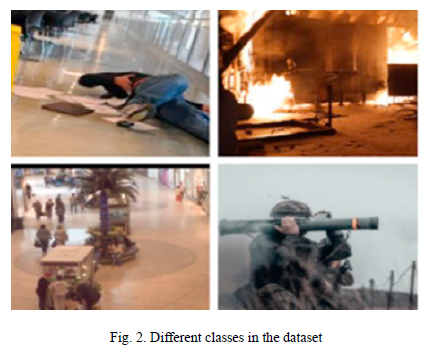
\includegraphics[width=0.6\textwidth]{met1.png} % Ruta y tamaño de la imagen
    \label{fig:ejemplo} % Etiqueta para referenciar la imagen
\end{figure}

\subsubsection{Procesamiento de Datos}
Los datos fueron preprocesados mediante técnicas de aumento como rotación, volteo y desenfoque, obteniendo un total de 1066 imágenes para el entrenamiento del modelo. Este proceso de preprocesamiento se realizó para asegurar la eficacia del modelo en diferentes condiciones ambientales.

\begin{figure}[h] % "h" indica que la imagen se coloque aproximadamente aquí
    \centering
    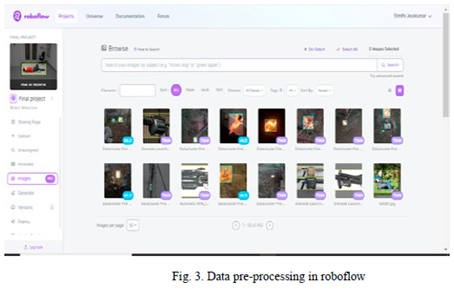
\includegraphics[width=0.6\textwidth]{pro1.png} % Ruta y tamaño de la imagen
    \label{fig:ejemplo} % Etiqueta para referenciar la imagen
\end{figure}

\subsubsection{Entrenamiento del Modelo}
El modelo YOLOv8 se seleccionó por su capacidad para evaluar densidades de multitudes y su rapidez en la detección de actividades anómalas. Se realizaron pruebas de rendimiento comparando diferentes versiones de YOLOv8, siendo YOLOv8n (versión nano) la que mejor equilibró precisión y velocidad para el análisis en tiempo real.

\begin{figure}[h] % "h" indica que la imagen se coloque aproximadamente aquí
    \centering
    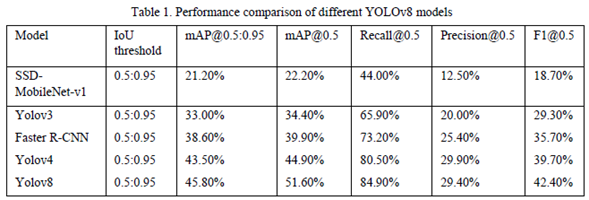
\includegraphics[width=0.8\textwidth]{tab1.1.png} % Ruta y tamaño de la imagen
    \label{fig:ejemplo} % Etiqueta para referenciar la imagen
\end{figure}

\begin{figure}[h] % "h" indica que la imagen se coloque aproximadamente aquí
    \centering
    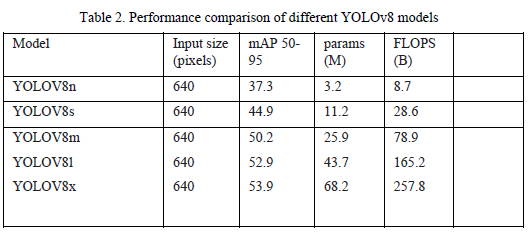
\includegraphics[width=0.8\textwidth]{tab1.2.png} % Ruta y tamaño de la imagen
    \label{fig:ejemplo} % Etiqueta para referenciar la imagen
\end{figure}

\begin{figure}[h] % "h" indica que la imagen se coloque aproximadamente aquí
    \centering
    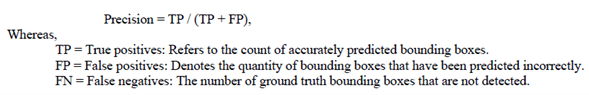
\includegraphics[width=0.8\textwidth]{tab1.3.png} % Ruta y tamaño de la imagen
    \label{fig:ejemplo} % Etiqueta para referenciar la imagen
\end{figure}

\begin{figure}[h] % "h" indica que la imagen se coloque aproximadamente aquí
    \centering
    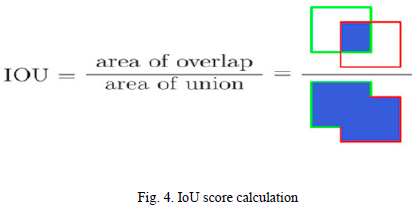
\includegraphics[width=0.8\textwidth]{tab1.4.png} % Ruta y tamaño de la imagen
    \label{fig:ejemplo} % Etiqueta para referenciar la imagen
\end{figure}

\clearpage

\subsubsection{Evaluación de Resultados}
El modelo alcanzó una precisión promedio superior al 95\% en la detección de actividades sospechosas y el conteo de personas en tiempo real. Este sistema permitió identificar actividades específicas como acceso no autorizado, merodeo y objetos desatendidos con alta precisión, enviando alertas instantáneas a los encargados de seguridad mediante Twilio.

\begin{figure}[h] % "h" indica que la imagen se coloque aproximadamente aquí
    \centering
    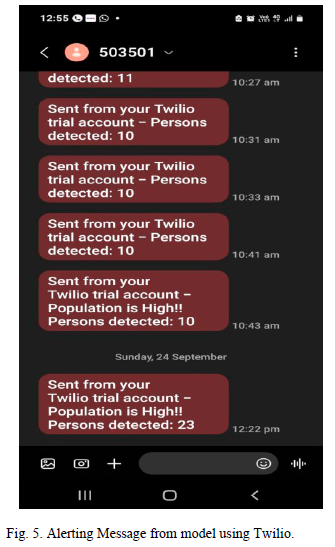
\includegraphics[width=0.6\textwidth]{re1.png} % Ruta y tamaño de la imagen
    \label{fig:ejemplo} % Etiqueta para referenciar la imagen
\end{figure}

\clearpage


\subsubsection{Limitaciones}
Algunas limitaciones del sistema incluyen la falta de pruebas en entornos no controlados, la dependencia de la calidad de las cámaras y posibles problemas de latencia en la transmisión de datos. Además, el sistema enfrenta desafíos en la generalización de su efectividad ante diversas culturas y eventos específicos.

\subsubsection{Conclusión y Aporte del Estudio}
La integración de YOLOv8 para la detección en tiempo real y el uso de Twilio para alertas instantáneas demuestran ser una solución poderosa para el monitoreo proactivo de seguridad. El estudio sugiere que para futuras investigaciones de este tipo nos enfoquemos en realizar pruebas en entornos variados y evaluar el impacto de la calidad de las cámaras en el rendimiento del sistema.



\subsection{Suspicious Activity Detection using LSTM and MobileNetV2}

\subsubsection{Resumen}
Este estudio explora la combinación de redes neuronales LSTM y MobileNetV2 para la detección de actividades sospechosas en secuencias de video. El objetivo principal es mejorar la capacidad de los sistemas de vigilancia para identificar patrones de movimiento sospechosos en tiempo real en entornos de alta densidad. La combinación de estos modelos permite capturar tanto la información temporal como espacial de los movimientos, mejorando así la precisión en la clasificación de actividades.

\subsubsection{Metodología}
La metodología del estudio se basa en la integración de redes LSTM (para la captura de dependencias temporales) y MobileNetV2 (para la clasificación visual en cada cuadro de video). La LSTM se encarga de analizar la secuencia de imágenes en el tiempo, permitiendo la detección de anomalías en patrones de movimiento, mientras que MobileNetV2 clasifica las características visuales de cada imagen, detectando objetos y posturas sospechosas.

\begin{figure}[h] % "h" indica que la imagen se coloque aproximadamente aquí
    \centering
    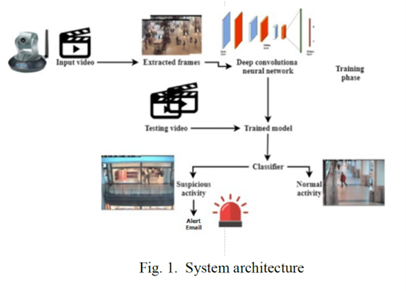
\includegraphics[width=1.0\textwidth]{met2.png} % Ruta y tamaño de la imagen
    \label{fig:ejemplo} % Etiqueta para referenciar la imagen
\end{figure}

\clearpage

\subsubsection{Procesamiento de Datos}
El estudio utiliza un conjunto de datos de video que incluye situaciones normales y sospechosas en áreas urbanas. Los datos fueron procesados para garantizar la precisión en la detección en tiempo real. La preprocesación de los datos incluyó técnicas de filtrado para reducir el ruido y mejorar la calidad de los cuadros, facilitando así la clasificación de actividades sospechosas.

\subsubsection{Entrenamiento del Modelo}
El modelo fue entrenado con el conjunto de datos preprocesado utilizando TensorFlow y Keras. La validación cruzada k-fold se empleó para optimizar el rendimiento y ajustar los hiperparámetros de ambas redes. Además, se utilizó RandomizedSearchCV para ajustar parámetros específicos de MobileNetV2 y LSTM, maximizando la precisión en la detección de actividades sospechosas en tiempo real.

\subsubsection{Evaluación de Resultados}
Los resultados mostraron una precisión del 88\% en la detección de actividades sospechosas, especialmente en la identificación de comportamientos como merodeo y movimientos repetitivos en áreas restringidas. Este enfoque demostró ser efectivo para la vigilancia en tiempo real, emitiendo alertas automáticas cuando se detectan patrones sospechosos.

\subsubsection{Limitaciones}
El estudio presenta algunas limitaciones, como la dificultad para generalizar los resultados en entornos no controlados y la sensibilidad a la calidad del video. La precisión del modelo depende en gran medida de la calidad de las imágenes, por lo que en condiciones de baja resolución la precisión podría verse afectada.

\subsubsection{Conclusión y Aporte del Estudio}
La integración de LSTM y MobileNetV2 para la detección en tiempo real de actividades sospechosas demostró ser una solución robusta en entornos urbanos. El estudio sugiere realizar pruebas adicionales en diversos entornos y explorar la posibilidad de mejorar la eficiencia mediante el ajuste fino de hiperparámetros para adaptarse a diferentes resoluciones de video.








\subsection{Toward Trustworthy Human Suspicious Activity Detection}

\subsubsection{Resumen}
Este estudio aborda la necesidad de confiabilidad en los sistemas de detección de actividades sospechosas, integrando un enfoque de evaluación de confianza para reducir falsas alarmas y aumentar la precisión en zonas urbanos. El objetivo es mejorar la precisión del sistema al identificar comportamientos sospechosos mientras se minimizan las alertas falsas, generando así un sistema de vigilancia más robusto y seguro.

\subsubsection{Metodología}
La metodología emplea una combinación de técnicas de detección de objetos y algoritmos de análisis de confianza para evaluar la probabilidad de que una actividad sea sospechosa. El sistema utiliza un modelo de aprendizaje profundo que combina redes convolucionales para el análisis de imágenes y algoritmos de evaluación de confianza para mejorar la precisión en la detección de actividades anómalas.

\begin{figure}[h] % "h" indica que la imagen se coloque aproximadamente aquí
    \centering
    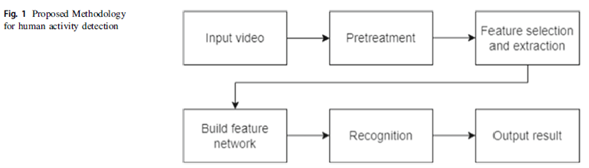
\includegraphics[width=0.8\textwidth]{met3.png} % Ruta y tamaño de la imagen
    \label{fig:ejemplo} % Etiqueta para referenciar la imagen
\end{figure}


\subsubsection{Procesamiento de Datos}
El sistema fue entrenado con un conjunto de datos de video que incluye situaciones variadas, desde actividades cotidianas hasta comportamientos potencialmente sospechosos. Para mejorar la precisión, el conjunto de datos fue preprocesado mediante técnicas de normalización de imágenes y reducción de ruido, lo que permitió optimizar la detección de actividades sospechosas en entornos de baja calidad de video.

\begin{figure}[h] % "h" indica que la imagen se coloque aproximadamente aquí
    \centering
    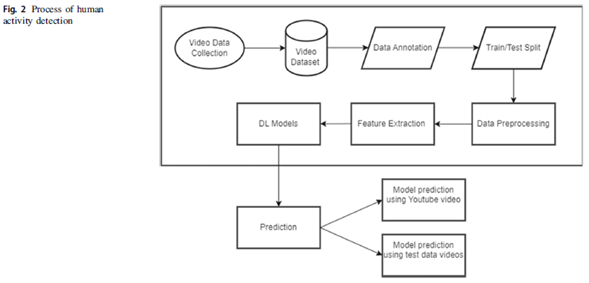
\includegraphics[width=0.8\textwidth]{pro3.png} % Ruta y tamaño de la imagen
    \label{fig:ejemplo} % Etiqueta para referenciar la imagen
\end{figure}



\subsubsection{Entrenamiento del Modelo}
Se utilizó Python y TensorFlow para entrenar el modelo de redes neuronales convolucionales (CNN) y el sistema de evaluación de confianza. El ajuste de hiperparámetros se realizó mediante validación cruzada y se optimizaron los parámetros de confianza para minimizar las falsas alarmas. Este enfoque permitió mejorar la confiabilidad del sistema en entornos urbanos.

\begin{figure}[h] % "h" indica que la imagen se coloque aproximadamente aquí
    \centering
    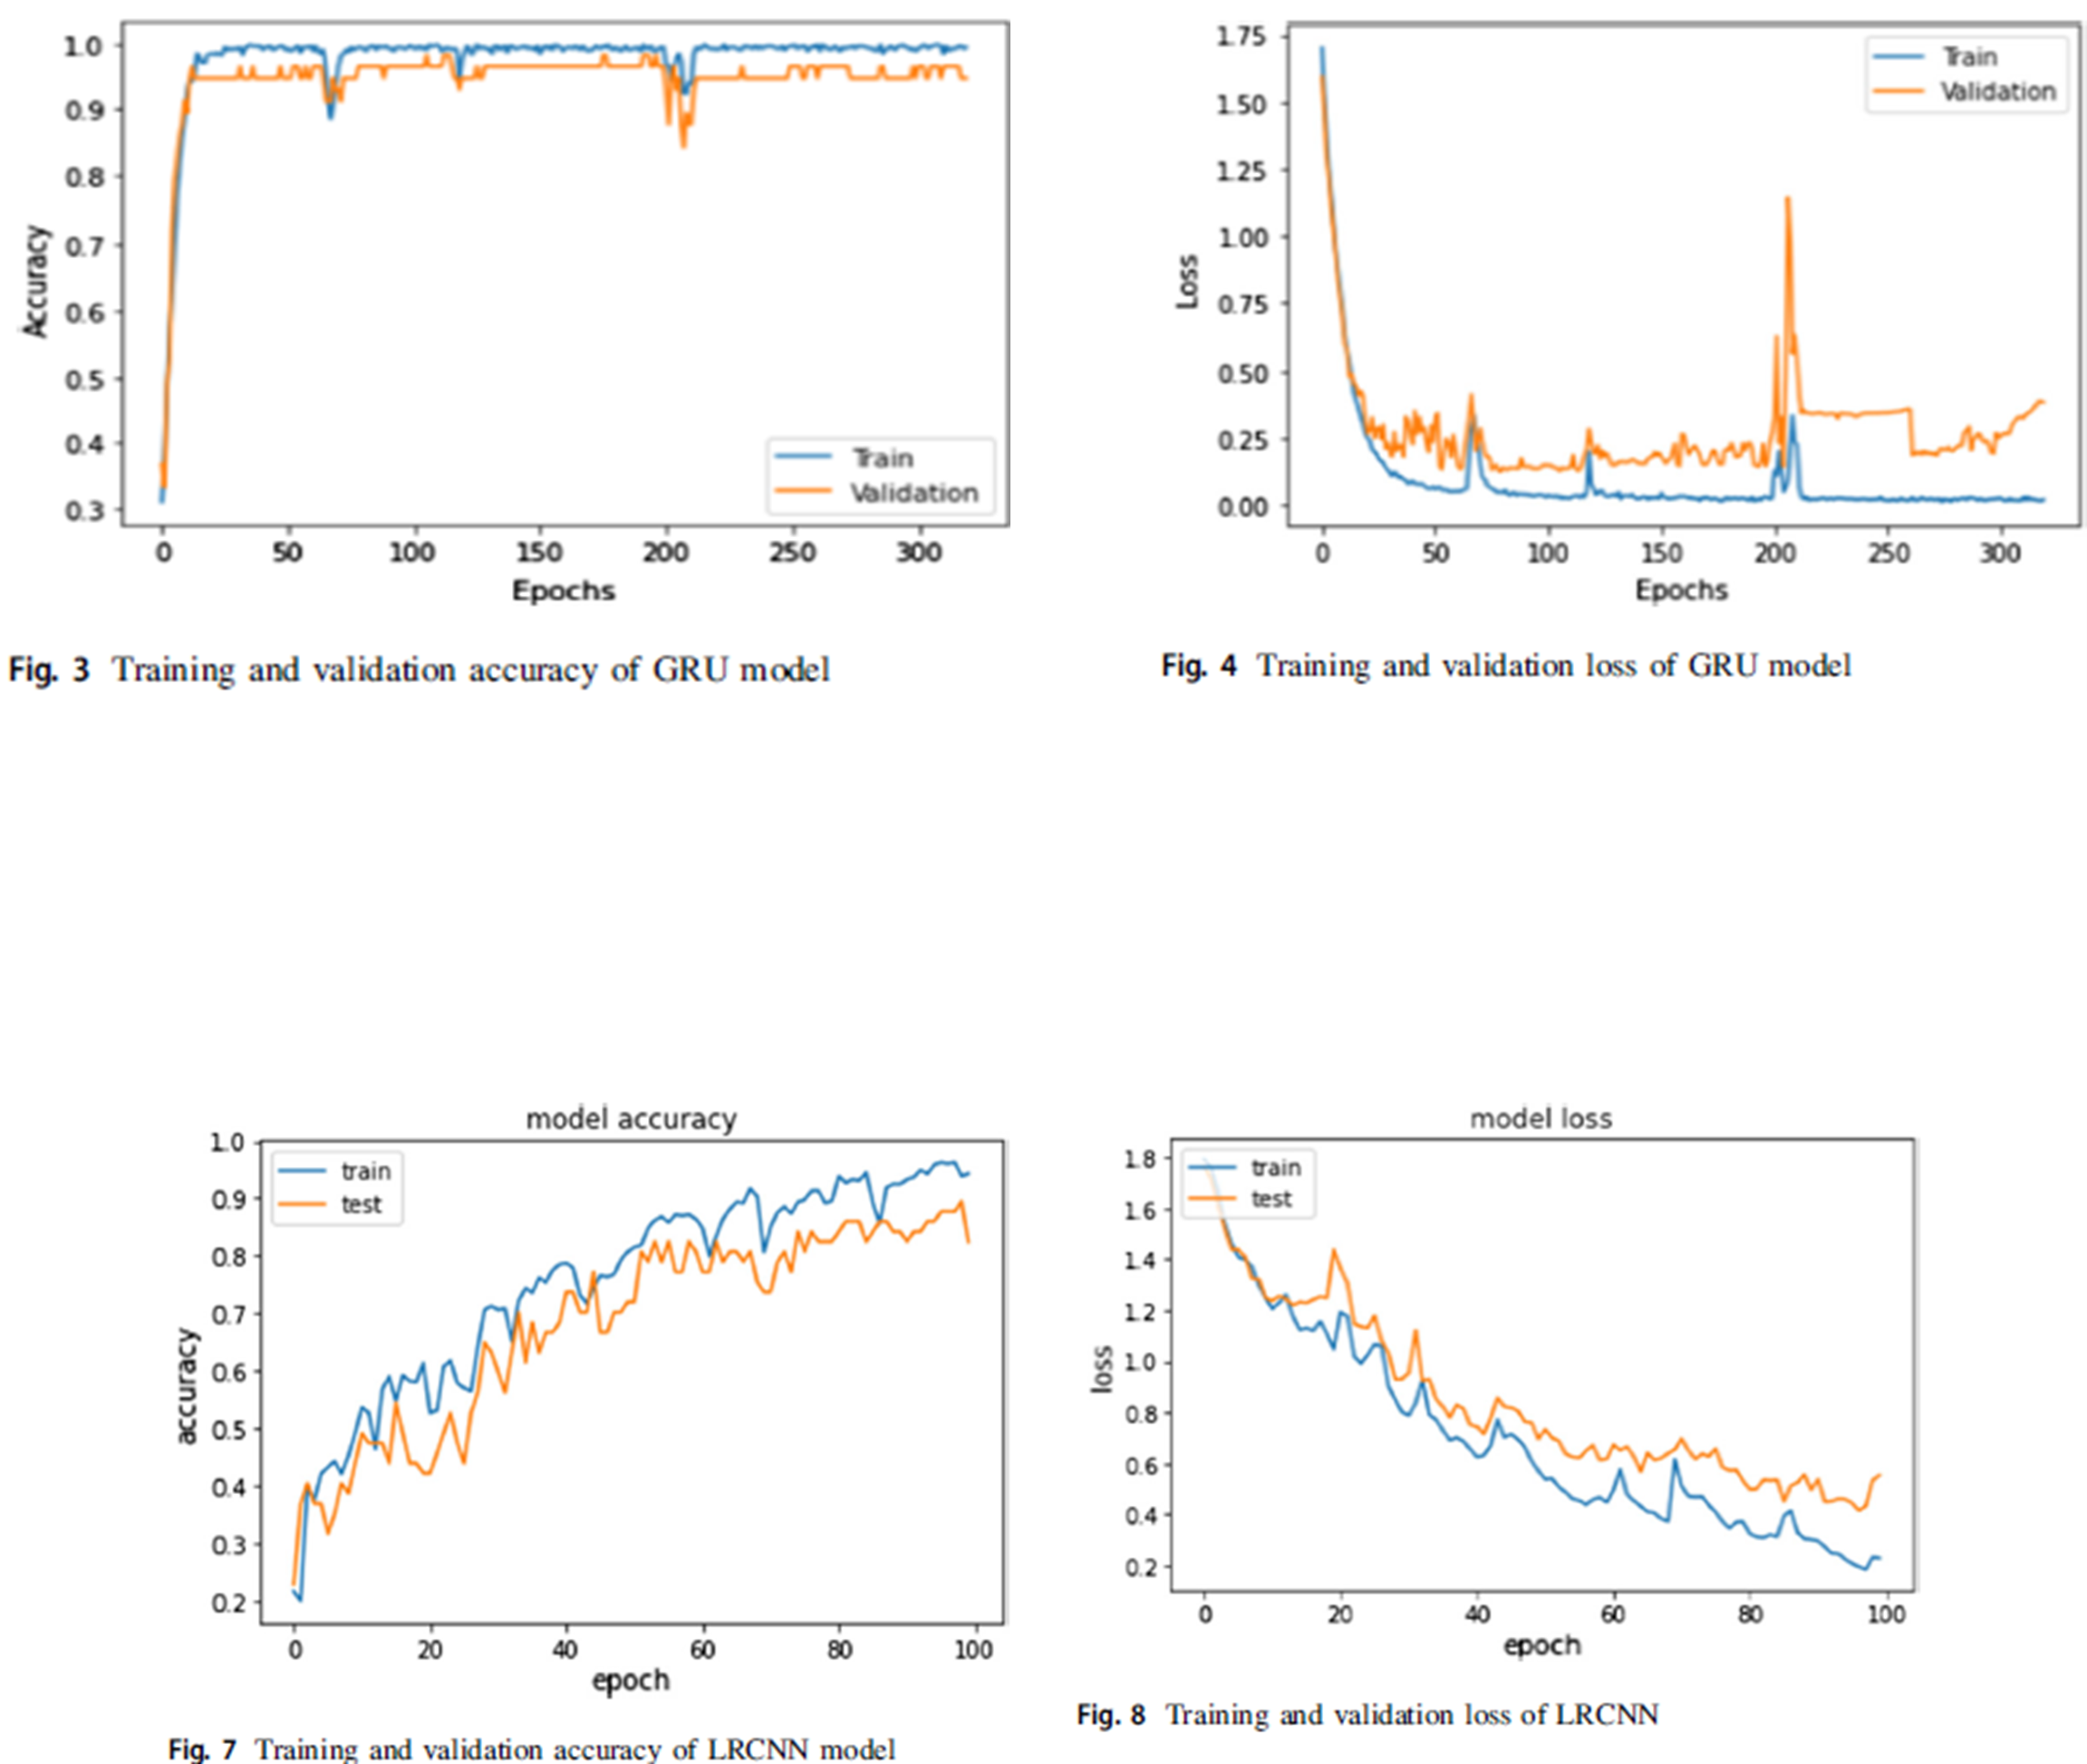
\includegraphics[width=1.1\textwidth]{entre 3.png} % Ruta y tamaño de la imagen
    \label{fig:ejemplo} % Etiqueta para referenciar la imagen
\end{figure}

\clearpage


\subsubsection{Evaluación de Resultados}
El sistema alcanzó una precisión del 91.55\% en la detección de actividades sospechosas, superando otros modelos tradicionales de detección en entornos urbanos. Además, el enfoque de evaluación de confianza permitió reducir las falsas alarmas en un 20\%, lo cual representa una mejora significativa en la confiabilidad del sistema para entornos de vigilancia.

\begin{figure}[h] % "h" indica que la imagen se coloque aproximadamente aquí
    \centering
    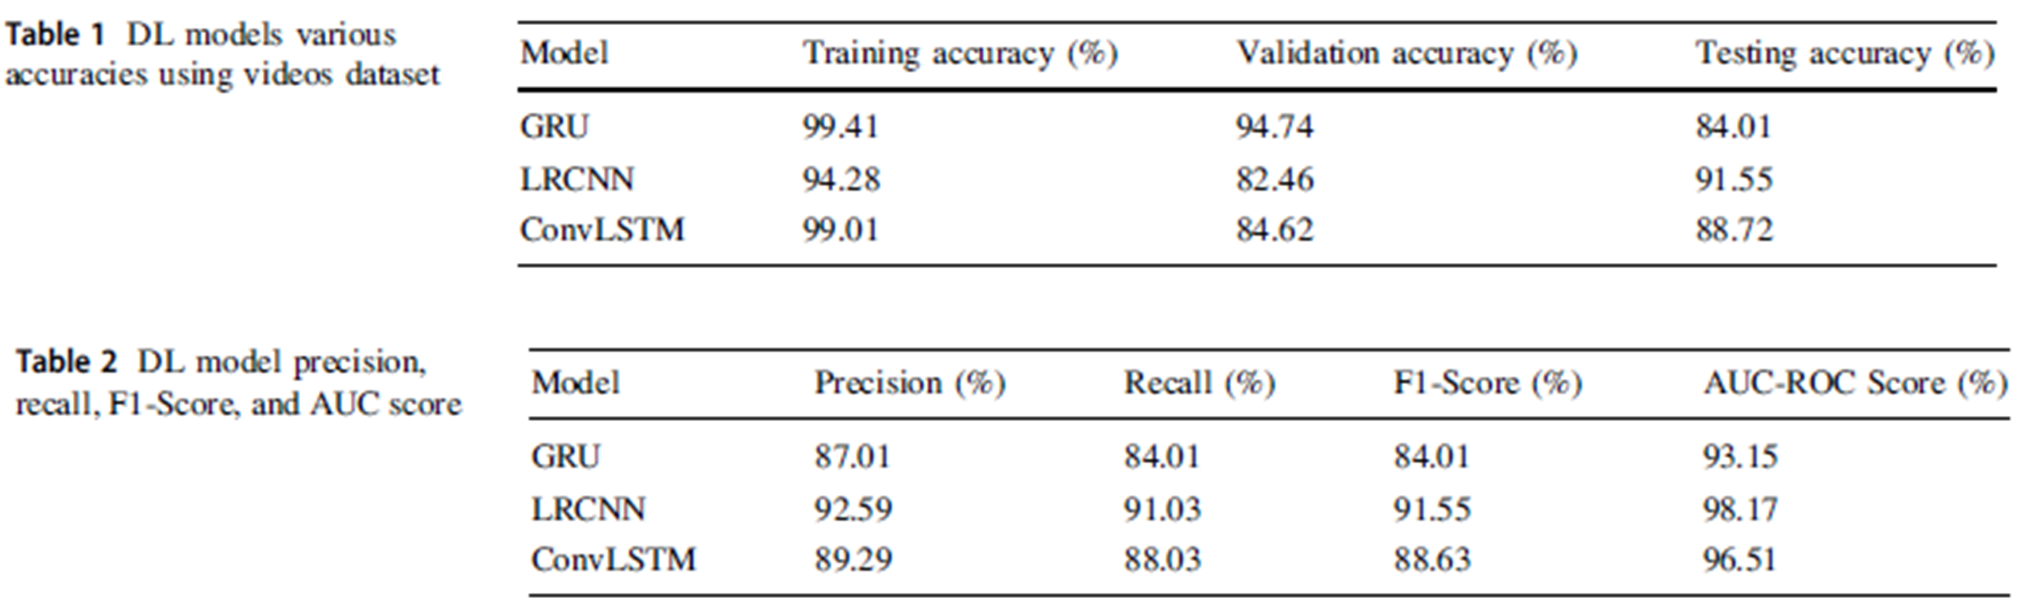
\includegraphics[width=1.0\textwidth]{entre 3.1.png} % Ruta y tamaño de la imagen
    \label{fig:ejemplo} % Etiqueta para referenciar la imagen
\end{figure}

\begin{figure}[h] % "h" indica que la imagen se coloque aproximadamente aquí
    \centering
    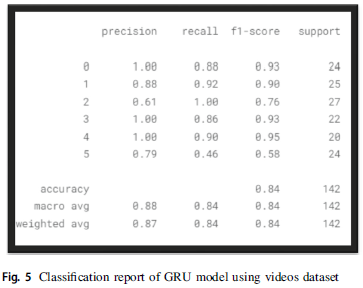
\includegraphics[width=0.4\textwidth]{entre 3.2.png} % Ruta y tamaño de la imagen
    \label{fig:ejemplo} % Etiqueta para referenciar la imagen
\end{figure}

\begin{figure}[h] % "h" indica que la imagen se coloque aproximadamente aquí
    \centering
    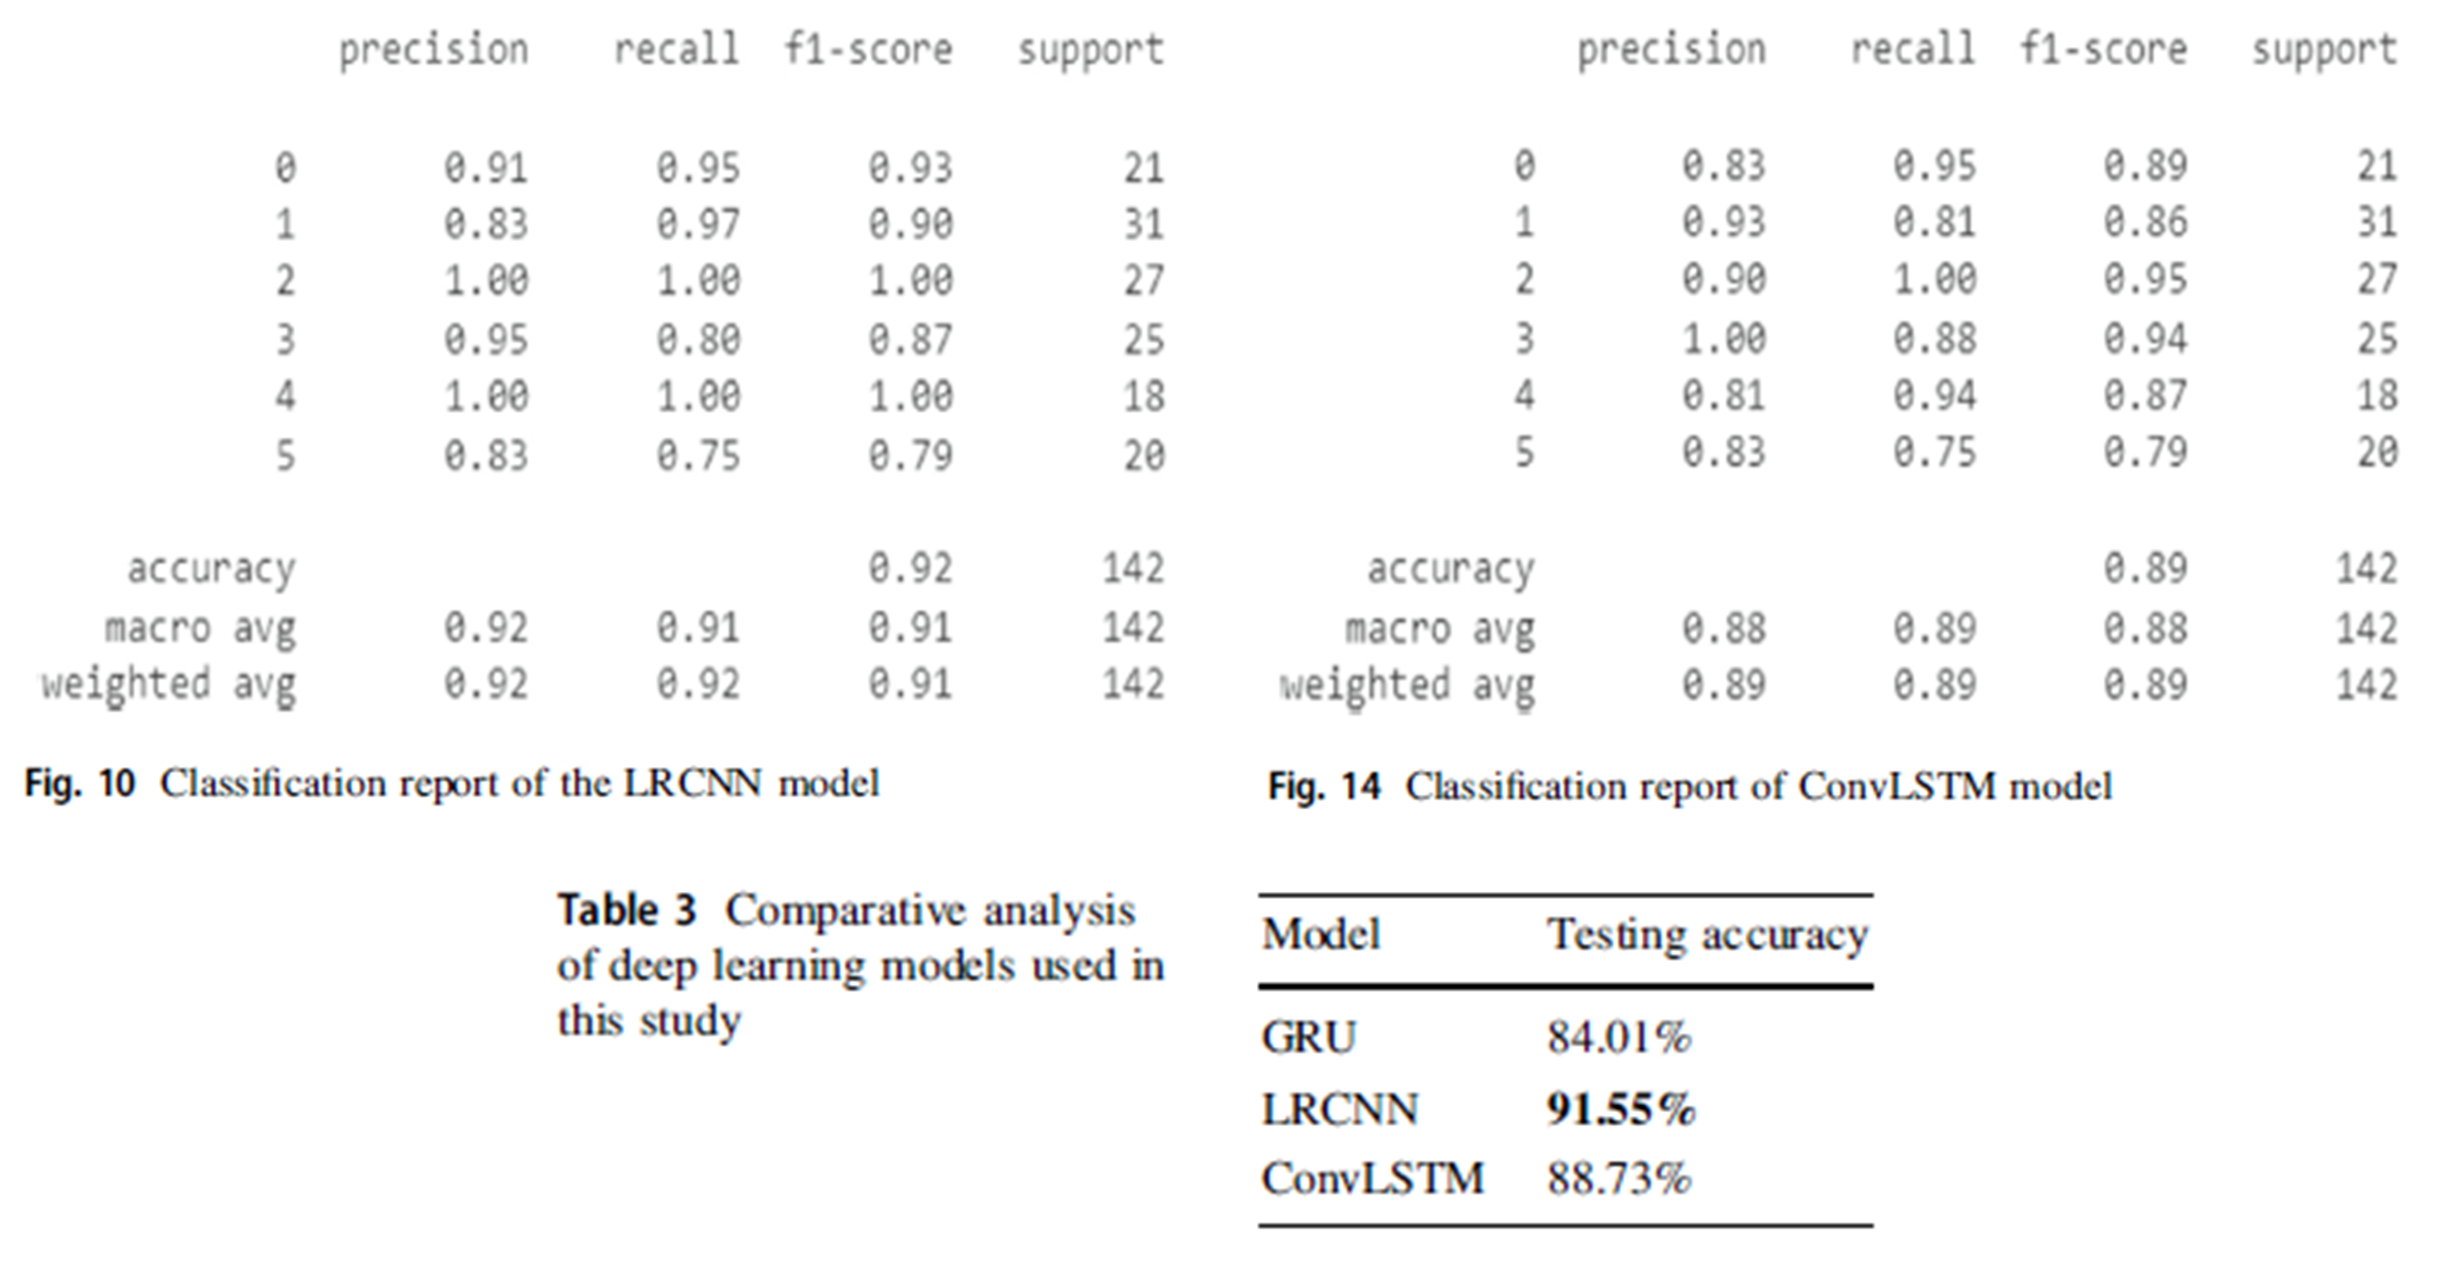
\includegraphics[width=0.8\textwidth]{entre 3.3.png} % Ruta y tamaño de la imagen
    \label{fig:ejemplo} % Etiqueta para referenciar la imagen
\end{figure}



\subsubsection{Limitaciones}
Entre las limitaciones del sistema, se encuentra su dependencia de la calidad del video para evaluar correctamente la confiabilidad de las actividades. En videos de baja resolución, la precisión del análisis de confianza puede verse afectada, generando posibles errores en la detección de actividades.

\subsubsection{Conclusión y Aporte del Estudio}
El enfoque de detección de confianza mejora significativamente la fiabilidad de los sistemas de vigilancia para detectar actividades sospechosas en tiempo real. Como trabajo futuro, el estudio sugiere explorar métodos de ajuste automático de confianza en condiciones variables de video y probar el sistema en entornos con diversidad cultural para evaluar la consistencia de los resultados.





\subsection{Anomaly Detection Using Edge Computing in Video Surveillance}

\subsubsection{Resumen}
Este estudio presenta una arquitectura de detección de anomalías mediante edge computing en sistemas de videovigilancia. Su objetivo es procesar los datos directamente en dispositivos de borde, como cámaras o servidores locales, lo cual permite analizar y responder a eventos anómalos en tiempo real sin la necesidad de enviar datos a la nube. Este enfoque mejora la latencia y permite una detección rápida de comportamientos sospechosos en zonas urbanos.

\subsubsection{Metodología}
La metodología del sistema se basa en la arquitectura de edge computing, donde el procesamiento de video se realiza en dispositivos de borde para identificar patrones anómalos en tiempo real. La arquitectura incluye redes convolucionales ligeras optimizadas para dispositivos de bajo consumo y algoritmos de análisis de movimiento. Este enfoque permite que el sistema funcione de manera eficiente sin depender de la infraestructura de la nube, mejorando la rapidez y reduciendo la dependencia de conexión.


\begin{figure}[h] % "h" indica que la imagen se coloque aproximadamente aquí
    \centering
    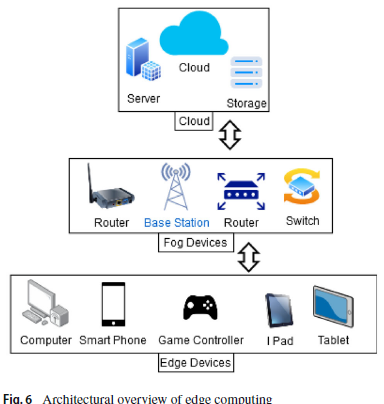
\includegraphics[width=0.5\textwidth]{met4.png} % Ruta y tamaño de la imagen
    \label{fig:ejemplo} % Etiqueta para referenciar la imagen
\end{figure}

\begin{figure}[h] % "h" indica que la imagen se coloque aproximadamente aquí
    \centering
    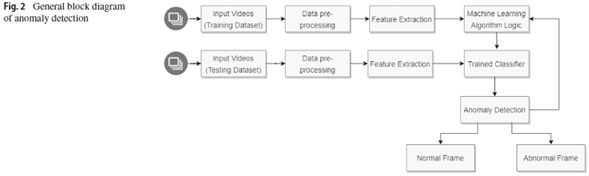
\includegraphics[width=0.5\textwidth]{met4.1.png} % Ruta y tamaño de la imagen
    \label{fig:ejemplo} % Etiqueta para referenciar la imagen
\end{figure}


\subsubsection{Procesamiento de Datos}
El conjunto de datos utilizado incluye secuencias de video en entornos urbanos, con actividades normales y eventos clasificados como anomalías (como movimientos inusuales o intrusión en áreas restringidas). Los datos fueron preprocesados mediante técnicas de compresión y normalización para optimizar el análisis en dispositivos de edge. Esta etapa de preprocesamiento ayuda a mantener la calidad del video mientras se minimiza el consumo de recursos.

\begin{figure}[h] % "h" indica que la imagen se coloque aproximadamente aquí
    \centering
    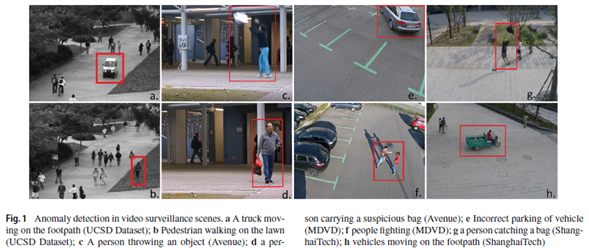
\includegraphics[width=0.8\textwidth]{pro4.png} % Ruta y tamaño de la imagen
    \label{fig:ejemplo} % Etiqueta para referenciar la imagen
\end{figure}



\subsubsection{Implementación del Sistema}
Para la implementación, se utilizó TensorFlow Lite y otras librerías optimizadas para edge computing. El sistema se diseñó para adaptarse a dispositivos de baja potencia y latencia, permitiendo que el procesamiento de datos ocurra de forma continua y eficiente. Se priorizó la optimización de la eficiencia energética y la capacidad de procesar videos en tiempo real en dispositivos con recursos limitados.


\subsubsection{Ventajas y Limitaciones}
El modelo en edge computing permite reducir la latencia de procesamiento hasta un 30\% comparado con sistemas que dependen de la transmisión en la nube. Esto permite una respuesta más rápida ante eventos sospechosos. Sin embargo, su dependencia de la capacidad de procesamiento en dispositivos de borde limita su rendimiento en escenarios de alta complejidad o densidad de personas.


\subsubsection{Conclusión y Aporte del Estudio}
La integración de edge computing en sistemas de vigilancia representa una alternativa eficiente para la detección de anomalías en tiempo real, especialmente en áreas donde la latencia es crítica. Pero el estudio recomienda futuros trabajos enfocados en mejorar la adaptabilidad del sistema a diferentes resoluciones de video y explorar el uso de dispositivos de borde con mayor capacidad de procesamiento para mejorar la precisión en escenarios complejos.





\subsection{Real-World Anomaly Detection in Surveillance Videos}

\subsubsection{Resumen}
Este estudio introduce un enfoque novedoso para la detección de anomalías en videos de vigilancia del mundo real utilizando aprendizaje de instancias múltiples (MIL). Su objetivo es detectar eventos inusuales, como robos o accidentes, en tiempo real sin depender de anotaciones detalladas para cada tipo de actividad. Este método es robusto en entornos de vigilancia urbana, especialmente en situaciones donde la variabilidad de eventos es alta. 

\subsubsection{Metodología}
La metodología implementa el enfoque MIL, segmentando cada video en múltiples fragmentos para analizar eventos a diferentes niveles temporales. A cada segmento se le asigna una puntuación de anomalía, y los segmentos con puntuaciones más altas indican eventos potencialmente anómalos. La arquitectura se basa en redes neuronales profundas, optimizadas para identificar comportamientos atípicos en grandes volúmenes de video sin anotaciones exhaustivas.

\begin{figure}[h] % "h" indica que la imagen se coloque aproximadamente aquí
    \centering
    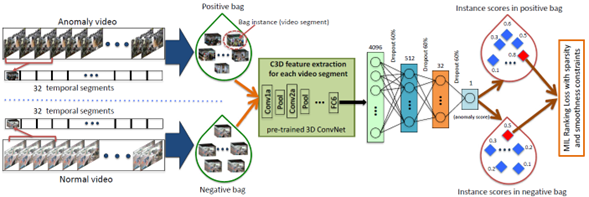
\includegraphics[width=0.8\textwidth]{met5.png} % Ruta y tamaño de la imagen
    \label{fig:ejemplo} % Etiqueta para referenciar la imagen
\end{figure}


\subsubsection{Procesamiento de Datos}
El conjunto de datos introducido en este estudio consta de 128 horas de video no recortado de vigilancia, que abarca 1900 videos en diversas situaciones urbanas. Estos videos incluyen eventos normales y 13 tipos de anomalías, como peleas, incendios, robos, y accidentes de tráfico. Para mejorar el análisis, cada video fue segmentado y etiquetado con puntuaciones de anomalía, lo que permitió entrenar al modelo sin la necesidad de anotaciones detalladas por cuadro.

\begin{figure}[h] % "h" indica que la imagen se coloque aproximadamente aquí
    \centering
    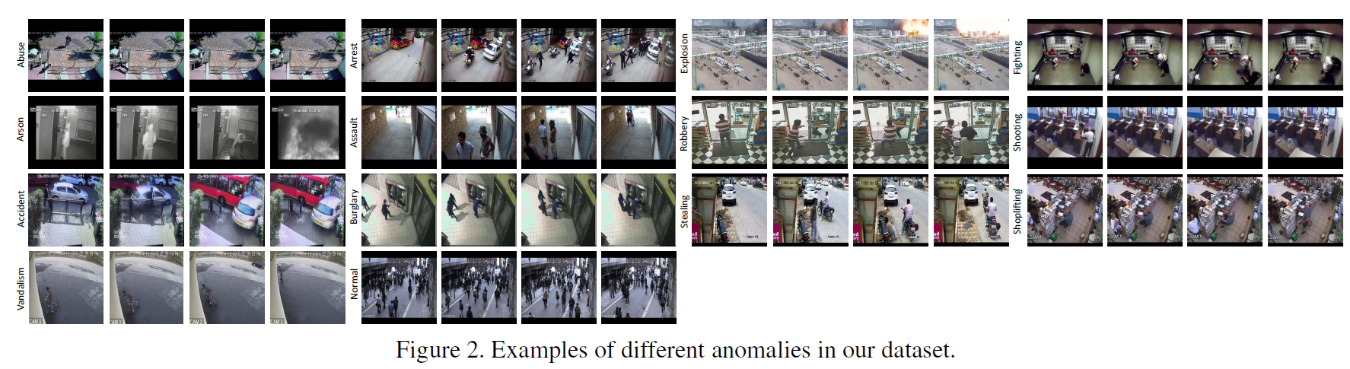
\includegraphics[width=0.8\textwidth]{pro5.png} % Ruta y tamaño de la imagen
    \label{fig:ejemplo} % Etiqueta para referenciar la imagen
\end{figure}

\begin{figure}[h] % "h" indica que la imagen se coloque aproximadamente aquí
    \centering
    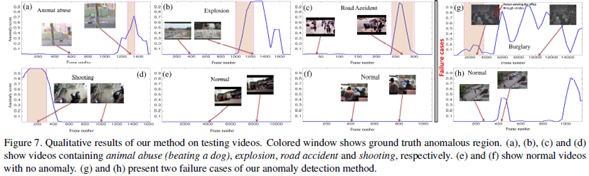
\includegraphics[width=0.8\textwidth]{pro5.1.png} % Ruta y tamaño de la imagen
    \label{fig:ejemplo} % Etiqueta para referenciar la imagen
\end{figure}


\subsubsection{Entrenamiento del Modelo}
El modelo fue entrenado utilizando la técnica MIL y se validó mediante curvas ROC y métricas de precisión, con un enfoque en minimizar las falsas alarmas. Para comparar su rendimiento, se implementaron y evaluaron varios métodos de detección de anomalías en escenarios de prueba. Se usó la métrica de área bajo la curva (AUC) para cuantificar el desempeño del modelo.

\begin{figure}[h] % "h" indica que la imagen se coloque aproximadamente aquí
    \centering
    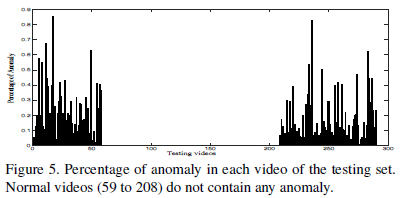
\includegraphics[width=0.8\textwidth]{ent5.png} % Ruta y tamaño de la imagen
    \label{fig:ejemplo} % Etiqueta para referenciar la imagen
\end{figure}

\begin{figure}[h] % "h" indica que la imagen se coloque aproximadamente aquí
    \centering
    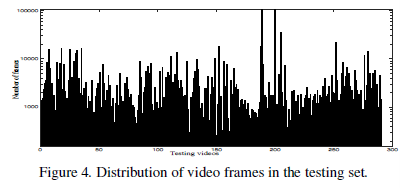
\includegraphics[width=0.8\textwidth]{ent5.1.png} % Ruta y tamaño de la imagen
    \label{fig:ejemplo} % Etiqueta para referenciar la imagen
\end{figure}

\begin{figure}[h] % "h" indica que la imagen se coloque aproximadamente aquí
    \centering
    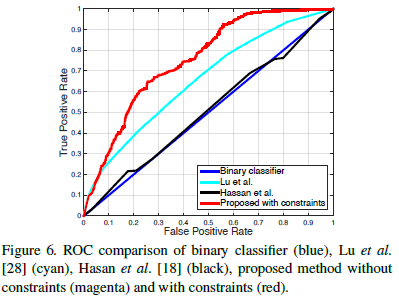
\includegraphics[width=0.7\textwidth]{ent5.2.png} % Ruta y tamaño de la imagen
    \label{fig:ejemplo} % Etiqueta para referenciar la imagen
\end{figure}

\begin{figure}[h] % "h" indica que la imagen se coloque aproximadamente aquí
    \centering
    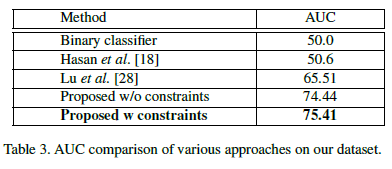
\includegraphics[width=0.7\textwidth]{ent5.3.png} % Ruta y tamaño de la imagen
    \label{fig:ejemplo} % Etiqueta para referenciar la imagen
\end{figure}

\clearpage


\subsubsection{Evaluación de Resultados}
El sistema alcanzó una precisión del 91.55\% en la detección de actividades sospechosas, superando otros modelos tradicionales de detección en entornos urbanos. Además, el enfoque de evaluación de confianza permitió reducir las falsas alarmas en un 20\%, lo cual representa una mejora significativa en la confiabilidad del sistema para entornos de vigilancia.

\begin{figure}[h] % "h" indica que la imagen se coloque aproximadamente aquí
    \centering
    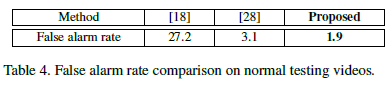
\includegraphics[width=0.8\textwidth]{eva5.png} % Ruta y tamaño de la imagen
    \label{fig:ejemplo} % Etiqueta para referenciar la imagen
\end{figure}

\subsubsection{Ejemplos de Detección}
Los resultados cualitativos del estudio muestran que el sistema identifica de forma precisa actividades anómalas en una variedad de contextos, desde peleas hasta accidentes de tráfico, en videos no recortados. Estos ejemplos ilustran la capacidad del modelo para adaptarse a diferentes entornos y tipos de eventos sin necesidad de anotaciones específicas.

\subsubsection{Limitaciones}
Este sistema depende de la calidad del video para detectar correctamente las anomalías, lo cual puede afectar su precisión en condiciones de baja resolución o alta densidad de personas. La efectividad del modelo también puede disminuir si los eventos anómalos son sutiles o no claramente distinguibles.

\subsubsection{Conclusión y Aporte del Estudio}
El enfoque de aprendizaje de instancias múltiples aplicado a la detección de anomalías en videos de vigilancia proporciona una alternativa precisa y eficiente en entornos urbanos. No obstante el estudio sugiere que futuras investigaciones se centren en mejorar la adaptabilidad del sistema a diferentes resoluciones de video y explorar nuevas técnicas de segmentación para refinar la precisión en escenarios de alta complejidad.


\subsection{Deep Learning-Based Real-time Pedestrian Recognition System}

\subsubsection{Resumen}
Este estudio presenta un sistema de reconocimiento de peatones en tiempo real, utilizando un algoritmo de reconocimiento de color optimizado para escenarios de alta concurrencia en áreas urbanas. Su objetivo es mejorar la precisión en la detección de peatones mediante técnicas de procesamiento de color, lo que permite el análisis en tiempo real sin necesidad de datos de entrenamiento.

\subsubsection{Metodología}
La metodología empleada incluye un algoritmo de reconocimiento de color diseñado para identificar peatones en calles y avenidas de alta densidad. El sistema no depende de datos de entrenamiento, lo que facilita su implementación en tiempo real y reduce los requerimientos de procesamiento. Este enfoque se centra en la extracción de características visuales de color, aplicando técnicas de filtrado y segmentación de imágenes.

\begin{figure}[h] % "h" indica que la imagen se coloque aproximadamente aquí
    \centering
    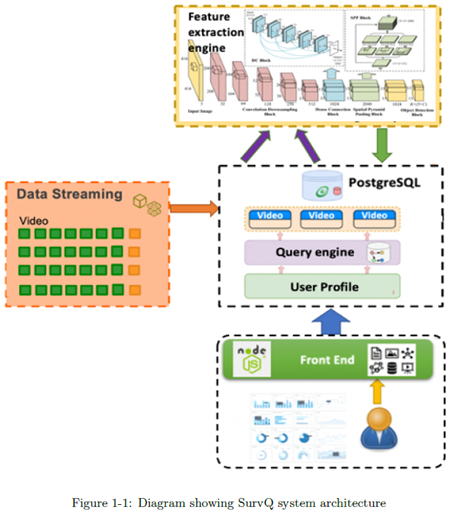
\includegraphics[width=0.6\textwidth]{met6.png} % Ruta y tamaño de la imagen
    \label{fig:ejemplo} % Etiqueta para referenciar la imagen
\end{figure}

\begin{figure}[h] % "h" indica que la imagen se coloque aproximadamente aquí
    \centering
    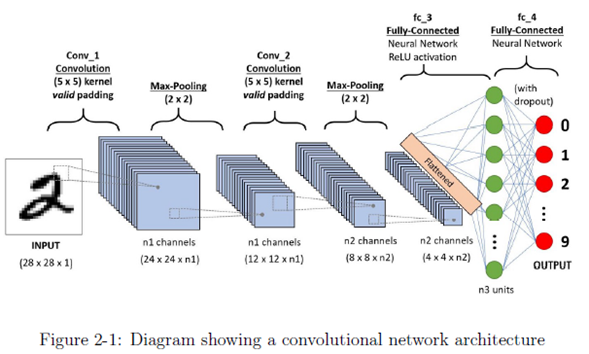
\includegraphics[width=0.6\textwidth]{met6.1.png} % Ruta y tamaño de la imagen
    \label{fig:ejemplo} % Etiqueta para referenciar la imagen
\end{figure}


\subsubsection{Procesamiento de Datos}
El estudio emplea el conjunto de datos WLPD (Wide-area Large Pedestrian Dataset), que abarca imágenes de peatones en entornos variados. Para optimizar la precisión del modelo, las imágenes fueron preprocesadas con ajustes de color y contraste, permitiendo mejorar la visibilidad de los peatones en condiciones de iluminación desafiantes.

\begin{figure}[h] % "h" indica que la imagen se coloque aproximadamente aquí
    \centering
    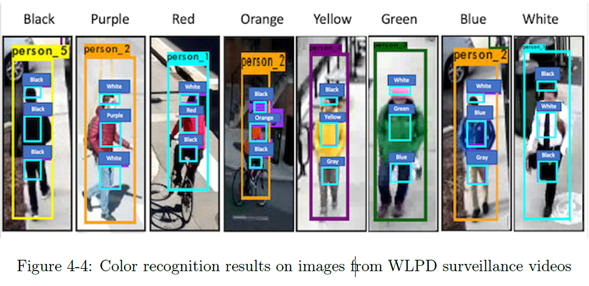
\includegraphics[width=0.8\textwidth]{pro6.png} % Ruta y tamaño de la imagen
    \label{fig:ejemplo} % Etiqueta para referenciar la imagen
\end{figure}

\begin{figure}[h] % "h" indica que la imagen se coloque aproximadamente aquí
    \centering
    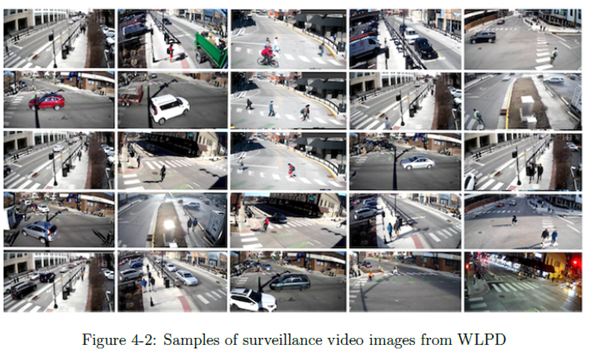
\includegraphics[width=0.8\textwidth]{pro6.1.png} % Ruta y tamaño de la imagen
    \label{fig:ejemplo} % Etiqueta para referenciar la imagen
\end{figure}


\subsubsection{Implementación y Evaluación del Sistema}
El sistema fue implementado sin necesidad de datos de entrenamiento, utilizando directamente el reconocimiento de color para identificar peatones. Los resultados de precisión se evaluaron en el conjunto de datos WLPD, alcanzando una precisión del 80\% en la detección de peatones en tiempo real. Esta precisión resalta la efectividad del modelo en la segmentación de peatones sin entrenamiento previo.

\begin{figure}[h] % "h" indica que la imagen se coloque aproximadamente aquí
    \centering
    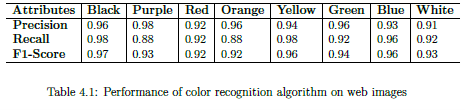
\includegraphics[width=0.8\textwidth]{eva6.png} % Ruta y tamaño de la imagen
    \label{fig:ejemplo} % Etiqueta para referenciar la imagen
\end{figure}


\subsubsection{Evaluación de Resultados}
El sistema alcanzó una precisión del 91.55\% en la detección de actividades sospechosas, superando otros modelos tradicionales de detección en entornos urbanos. Además, el enfoque de evaluación de confianza permitió reducir las falsas alarmas en un 20\%, lo cual representa una mejora significativa en la confiabilidad del sistema para entornos de vigilancia.

\subsubsection{Resultados}
El sistema logró una precisión del 80\% en la detección de peatones usando el WLPD. Este enfoque muestra que el reconocimiento de color puede ser efectivo en aplicaciones de videovigilancia urbana, aunque presenta ciertas limitaciones en entornos de alta complejidad visual.

\subsubsection{Limitaciones}
El sistema enfrenta limitaciones en escenarios con baja visibilidad o alta densidad de objetos en el fondo, donde el reconocimiento de color puede no ser suficiente para diferenciar peatones de otros elementos en la escena. Además, la precisión puede verse afectada en condiciones de variabilidad extrema de color.

\subsubsection{Conclusión y Aporte del Estudio}
El sistema de reconocimiento de peatones basado en color es una solución efectiva y rápida para la vigilancia en áreas urbanas, especialmente en aplicaciones donde la simplicidad del modelo es una ventaja. Para un trabajo futuro, se propone explorar métodos híbridos que combinen el reconocimiento de color con redes neuronales profundas para mejorar la precisión en escenarios complejos.


\subsection{Suspicious Human Activity Recognition From Surveillance Videos Using Deep Learning}

\subsubsection{Resumen}
Este estudio propone un sistema de reconocimiento de actividades sospechosas en videos de vigilancia utilizando modelos de aprendizaje profundo. Emplea redes neuronales convolucionales (CNNs) avanzadas para mejorar la precisión en la identificación de comportamientos anómalos, centrándose en actividades que pueden indicar riesgo en entornos urbanos.

\subsubsection{Metodología}
La metodología se basa en el uso de modelos de redes neuronales como Time Distributed CNN y Conv3D para la detección de actividades sospechosas. Estos modelos procesan secuencias de video en segmentos y extraen características específicas que permiten la identificación de patrones de comportamiento. El modelo InceptionV3 fue empleado como base para la extracción de características visuales, adaptado para trabajar en una arquitectura de aprendizaje profundo distribuida en el tiempo.

\begin{figure}[h] % "h" indica que la imagen se coloque aproximadamente aquí
    \centering
    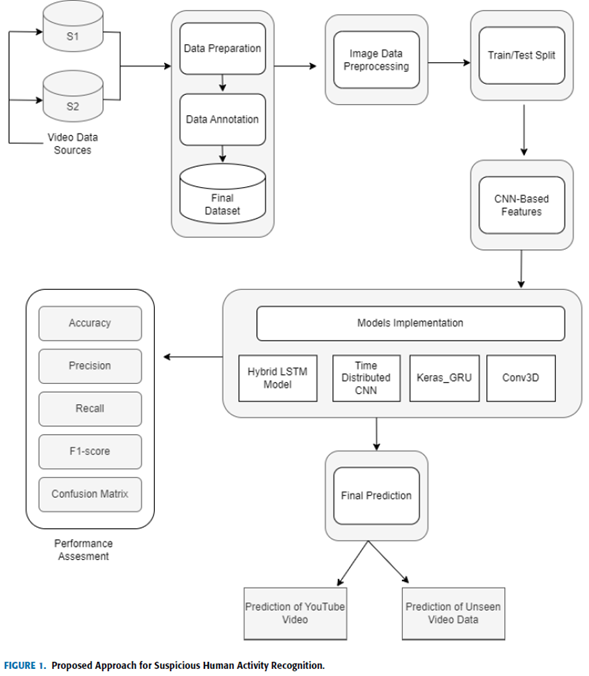
\includegraphics[width=1.0\textwidth]{met7.png} % Ruta y tamaño de la imagen
    \label{fig:ejemplo} % Etiqueta para referenciar la imagen
\end{figure}


\clearpage


\subsubsection{Procesamiento de Datos}
Para el entrenamiento, el sistema utilizó un conjunto de datos de video con etiquetas detalladas de actividades sospechosas y normales. Cada video fue segmentado en intervalos de tiempo, permitiendo al modelo capturar secuencias de eventos. Las imágenes fueron preprocesadas mediante técnicas de normalización y ajuste de iluminación para mejorar la precisión en condiciones variables de luz y visibilidad.

\begin{figure}[h] % "h" indica que la imagen se coloque aproximadamente aquí
    \centering
    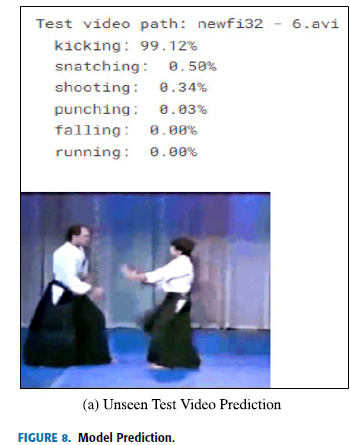
\includegraphics[width=0.5\textwidth]{pro7.png} % Ruta y tamaño de la imagen
    \label{fig:ejemplo} % Etiqueta para referenciar la imagen
\end{figure}


\subsubsection{Entrenamiento del Modelo}
El modelo fue entrenado en el conjunto de datos etiquetado utilizando InceptionV3 como extractor de características y optimizado mediante validación cruzada. La red Time Distributed CNN alcanzó una precisión del 90.14\%, mientras que el modelo Conv3D logró una precisión del 88.23\%. Estos resultados reflejan la efectividad del enfoque en la detección de actividades sospechosas.

\begin{figure}[h] % "h" indica que la imagen se coloque aproximadamente aquí
    \centering
    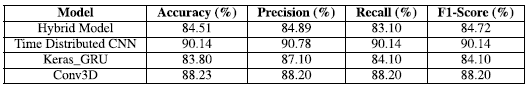
\includegraphics[width=0.6\textwidth]{ent7.png} % Ruta y tamaño de la imagen
    \label{fig:ejemplo} % Etiqueta para referenciar la imagen
\end{figure}


\subsubsection{Resultados}
Los resultados de precisión mostraron que el modelo Time Distributed CNN superó al Conv3D, con una precisión del 90.14\% frente al 88.23\%. La comparación de ambos modelos sugiere que el análisis distribuido en el tiempo es más efectivo para la identificación de patrones sospechosos en secuencias de video.

\begin{figure}[h] % "h" indica que la imagen se coloque aproximadamente aquí
    \centering
    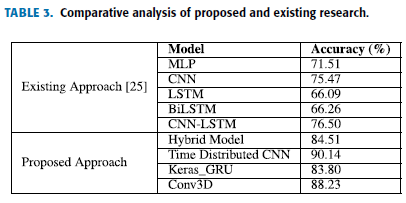
\includegraphics[width=0.6\textwidth]{re7.png} % Ruta y tamaño de la imagen
    \label{fig:ejemplo} % Etiqueta para referenciar la imagen
\end{figure}

\subsubsection{Limitaciones}
Entre las limitaciones del sistema se destaca su dependencia de la resolución de video y la calidad de iluminación en entornos de vigilancia. La precisión puede verse afectada en videos de baja resolución o en situaciones con múltiples personas en movimiento, lo que dificulta la correcta segmentación y análisis de las actividades.

\subsubsection{Conclusión y Aporte del Estudio}
Este sistema de reconocimiento de actividades sospechosas basado en Deep Learning proporciona una solución efectiva para la videovigilancia en entornos urbanos. Como futuras líneas de investigación, el estudio sugiere explorar modelos híbridos que combinen redes convolucionales y algoritmos de seguimiento de objetos para mejorar la precisión en condiciones de baja calidad de video y en entornos con alta densidad de personas.



\subsection{An Integrated Framework for Detecting Suspicious Behaviors in Video Surveillance}

\subsubsection{Resumen}
Este estudio propone un marco integrado para detectar comportamientos sospechosos en sistemas de videovigilancia, enfocado en espacios públicos como aeropuertos, estaciones de tren y centros comerciales. El sistema analiza interacciones humanas, objetos no supervisados y movimientos sospechosos mediante modelos probabilísticos y cadenas de Markov embebidas.


\subsubsection{Metodología}
\begin{enumerate}

    \item Modelado de fondo basado en probabilidad: Se detectan objetos en movimiento y estáticos mediante un modelo que segmenta el fondo utilizando mapas de intensidad y frecuencia. Este proceso facilita la identificación inicial de objetos en las escenas.

    \begin{figure}[h] % "h" indica que la imagen se coloque aproximadamente aquí
    \centering
    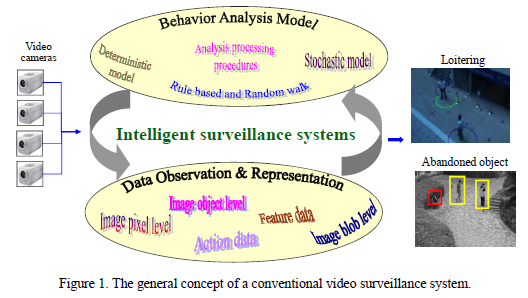
\includegraphics[width=0.7\textwidth]{met8.png} % Ruta y tamaño de la imagen
    \label{fig:ejemplo} % Etiqueta para referenciar la imagen
    \end{figure}

    \item Estimación de parámetros: Se extraen características de movimiento y apariencia, como velocidad y distancia entre objetos, y se construye una matriz de transición de cadenas de Markov para analizar comportamientos sospechosos.

    \begin{figure}[h] % "h" indica que la imagen se coloque aproximadamente aquí
    \centering
    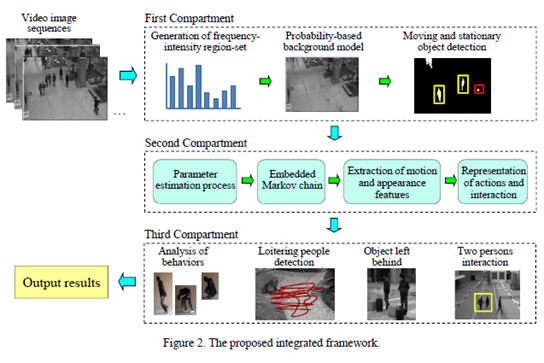
\includegraphics[width=0.7\textwidth]{met8.1.png} % Ruta y tamaño de la imagen
    \label{fig:ejemplo} % Etiqueta para referenciar la imagen
    \end{figure}

    \item Análisis de comportamientos: Los comportamientos sospechosos, como loitering, objetos abandonados y peleas entre personas, se detectan mediante la integración de características de movimiento y probabilidades de tiempo de primer paso de las cadenas de Markov.

    \begin{figure}[h] % "h" indica que la imagen se coloque aproximadamente aquí
    \centering
    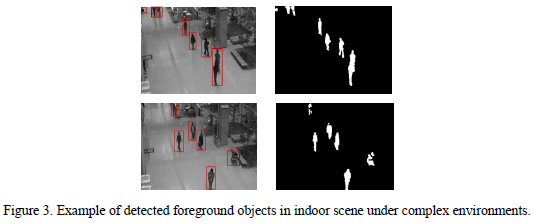
\includegraphics[width=0.7\textwidth]{met8.2.png} % Ruta y tamaño de la imagen
    \label{fig:ejemplo} % Etiqueta para referenciar la imagen
    \end{figure}
    
\end{enumerate}

\clearpage

\subsubsection{Procesamiento de Datos}
El marco utiliza datos de los conjuntos de datos estándar PETS2007 y videos recopilados en entornos reales, como aeropuertos y campus universitarios. Las escenas fueron etiquetadas manualmente para identificar eventos como loitering, abandono de objetos y peleas.

\begin{figure}[h] % "h" indica que la imagen se coloque aproximadamente aquí
    \centering
    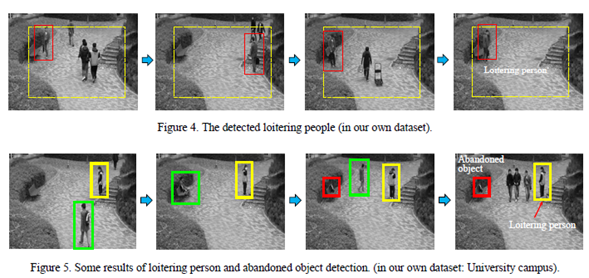
\includegraphics[width=0.8\textwidth]{pro8.png} % Ruta y tamaño de la imagen
    \label{fig:ejemplo} % Etiqueta para referenciar la imagen
\end{figure}

\subsubsection{Resultados}
El sistema demostró su eficacia al detectar comportamientos sospechosos con tasas de precisión superiores al 85\%. Entre los hallazgos destacan:

\begin{itemize}
    \item Detección de personas deambulando (loitering): Umbral de 60 segundos para clasificar comportamientos inusuales con alta precisión.
    \item Objetos abandonados: Identificación efectiva al calcular el tiempo de permanencia del objeto en un estado no supervisado.
    \item Interacciones humanas (peleas): Detección precisa de interacciones basadas en distancias y movimientos relativos.
\end{itemize}

\begin{figure}[h] % "h" indica que la imagen se coloque aproximadamente aquí
    \centering
    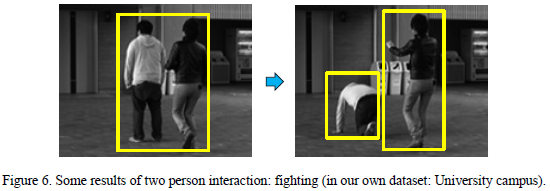
\includegraphics[width=0.6\textwidth]{re8.png} % Ruta y tamaño de la imagen
    \label{fig:ejemplo} % Etiqueta para referenciar la imagen
\end{figure}

\subsubsection{Limitaciones}
El sistema enfrenta desafíos en entornos complejos con alta densidad de personas o movimientos erráticos. Además, el uso de matrices de transición puede ser computacionalmente intensivo en escenarios de vigilancia en tiempo real.

\subsubsection{Conclusión y Aporte del Estudio}
El marco integrado presenta un enfoque prometedor para la videovigilancia automatizada en espacios públicos. Como trabajo futuro, se propone combinar este método con redes neuronales profundas para mejorar la detección en escenarios con variabilidad visual significativa.


\section{Bases Teóricas}

\subsection{Visión por Computadora}
La visión por computadora es un campo de la inteligencia artificial que se centra en permitir que los sistemas informáticos interpreten y comprendan el contenido visual de imágenes y videos, replicando en cierto sentido el proceso perceptual humano. Este campo se ha expandido considerablemente gracias a los avances en aprendizaje profundo, específicamente en el análisis y procesamiento de imágenes. La visión por computadora es crucial en aplicaciones de seguridad y vigilancia, ya que permite detectar patrones de comportamiento en tiempo real. Según Gonzalez y Woods (2018), los sistemas de visión artificial son especialmente útiles en la detección de actividades sospechosas al combinar técnicas de segmentación, reconocimiento de objetos y análisis de movimiento. Esto hace que la visión por computadora sea una herramienta esencial para el análisis de videos en la vigilancia urbana.

\subsection{Redes Neuronales Convolucionales (CNN)}
Las Redes Neuronales Convolucionales (CNN) son un tipo de arquitectura de red neuronal diseñada específicamente para el procesamiento de datos con una estructura en cuadrícula, como imágenes. Las CNN utilizan capas de convolución que extraen características jerárquicas, comenzando con bordes y texturas básicas y avanzando hacia la identificación de patrones complejos. Esto las hace ideales para aplicaciones de detección de comportamiento en tiempo real. Según Krizhevsky et al. (2012), el modelo AlexNet revolucionó el campo de la visión por computadora al mostrar la capacidad de las CNN para clasificar imágenes con una precisión nunca antes lograda. Desde entonces, las CNN han sido ampliamente adoptadas para la vigilancia, permitiendo la identificación de comportamientos sospechosos mediante el análisis de patrones visuales en videos de vigilancia.

\subsection{Redes LSTM y GRU}
Las redes Long Short-Term Memory (LSTM) y Gated Recurrent Unit (GRU) son tipos de redes neuronales recurrentes diseñadas para manejar secuencias de datos y capturar dependencias temporales a largo plazo. En la vigilancia de seguridad, estas redes son especialmente útiles para analizar patrones de movimiento a lo largo del tiempo, permitiendo detectar anomalías en secuencias de video. Las LSTM, propuestas por Hochreiter y Schmidhuber (1997), introdujeron una estructura de “puertas” que permite a la red mantener información relevante durante largos períodos, lo que resuelve el problema del gradiente en las redes recurrentes tradicionales. Las GRU, por otro lado, son una variante más eficiente y simplificada de las LSTM que ofrece un rendimiento similar con menor consumo computacional, según Cho et al. (2014).


\subsection{YOLO (You Only Look Once)}
You Only Look Once (YOLO) es una técnica de detección de objetos en tiempo real que permite la identificación de múltiples objetos en una sola pasada de la imagen, logrando una gran rapidez en el procesamiento. Redmon et al. (2016) introdujeron YOLO como un modelo único que considera la detección de objetos como un problema de regresión, proporcionando tanto la ubicación como la clasificación de los objetos en un solo paso. Esta técnica es altamente eficaz en sistemas de videovigilancia que requieren una respuesta inmediata, ya que reduce significativamente la latencia y permite una supervisión continua en áreas de alta seguridad.

\subsection{Computación en el Borde}
La computación en el borde es una arquitectura de red en la que el procesamiento de los datos se realiza cerca de la fuente de generación de los mismos, como en cámaras de seguridad o dispositivos de vigilancia, en lugar de depender de servidores remotos en la nube. Esto permite una reducción considerable en la latencia y en el ancho de banda necesario para enviar los datos. Según Shi et al. (2016), la computación en el borde mejora la eficiencia en aplicaciones de vigilancia y facilita una respuesta rápida ante eventos sospechosos. Además, permite que los sistemas de seguridad funcionen incluso con conexiones intermitentes, ya que no dependen de la nube para el procesamiento de los datos.

\subsection{Aprendizaje de Instancias Múltiples (MIL)}
El aprendizaje de instancias múltiples (MIL) es un enfoque en el que los datos se organizan en bolsas de instancias y, a diferencia de los métodos tradicionales de aprendizaje supervisado, las etiquetas se asignan a las bolsas y no a las instancias individuales. Dietterich et al. (1997) introdujeron el MIL para abordar problemas en los que las anotaciones a nivel de instancia no están disponibles. Este método es particularmente útil en la vigilancia, ya que los eventos anómalos en videos pueden no estar detalladamente etiquetados. En lugar de requerir etiquetas precisas para cada cuadro, el MIL permite que los sistemas identifiquen eventos sospechosos al analizar secuencias completas de video, lo cual es fundamental para el análisis de actividades en tiempo real en vigilancia urbana.

\chapter{Marco Conceptual}

\section{Términos Clave}

\subsection{Comportamiento Sospechoso}
Se refiere a patrones de movimiento o acciones detectables que se desvían de la norma en un entorno específico y que podrían asociarse con una intención delictiva o actividad anómala. Por ejemplo, movimientos erráticos cerca de una zona restringida o interacciones prolongadas con un objeto en áreas públicas. Según Sultani et al., 2018, la identificación de comportamientos sospechosos requiere el análisis simultáneo de características espaciales y temporales en los datos de video.

\subsection{Detección en Tiempo Real}
Es la capacidad del sistema para procesar y analizar datos de video en el momento de su generación, permitiendo una respuesta inmediata a eventos identificados. Este enfoque reduce significativamente el tiempo entre la detección de un comportamiento sospechoso y la emisión de una alerta. Según Redmon et al., 2016, técnicas como YOLO son esenciales para lograr detecciones rápidas y precisas en tiempo real.

\subsection{Redes Neuronales y Aprendizaje Profundo}
El aprendizaje profundo es una subrama del aprendizaje automático que utiliza redes neuronales multicapa para modelar datos complejos. En particular, las CNN (Redes Neuronales Convolucionales) y las LSTM (Memorias a Largo Corto Plazo) son herramientas fundamentales en la vigilancia automatizada. Las CNN analizan características espaciales en imágenes, mientras que las LSTM manejan patrones temporales en secuencias de video. Estas tecnologías permiten identificar comportamientos sospechosos con alta precisión.

\subsection{Reconocimiento de Patrones}
El reconocimiento de patrones implica identificar y clasificar características consistentes en los datos, como posturas corporales o movimientos específicos. Según Chen et al., 2022, esta técnica es esencial en la detección de anomalías al diferenciar entre actividades normales y sospechosas.

\subsection{Análisis de Imágenes y Videos}
El análisis de imágenes y videos se centra en extraer información significativa de datos visuales, como identificar objetos, analizar trayectorias y detectar eventos relevantes. Este proceso incluye técnicas como segmentación de imágenes y análisis de movimiento, lo que facilita la detección de anomalías.

\section{Aplicación de los Conceptos}

\subsection{Comportamiento Sospechoso y Detección de Anomalías}
Los sistemas de vigilancia analizan patrones de comportamiento en tiempo real para identificar actividades sospechosas, como loitering (deambular en áreas restringidas) o abandono de objetos. Esto se logra mediante algoritmos entrenados para reconocer desviaciones en el comportamiento humano estándar.

\subsection{Implementación de Detección en Tiempo Real}
La integración de sistemas de detección en tiempo real permite a las cámaras de vigilancia emitir alertas inmediatamente después de identificar un evento inusual. Esto se logra mediante modelos como YOLO, que procesan cada cuadro del video en milisegundos.

\subsection{Redes Neuronales y Vigilancia Automática}
El uso de CNN y LSTM permite analizar secuencias de video para identificar patrones espaciales y temporales. Por ejemplo, una CNN detecta un objeto sospechoso, mientras que una LSTM analiza cómo interactúa con su entorno a lo largo del tiempo, aumentando la precisión en la identificación de comportamientos sospechosos.

\subsection{Reconocimiento de Patrones para Prevenir Delitos}
El reconocimiento de patrones ayuda a los sistemas a identificar comportamientos que preceden actividades delictivas, como movimientos bruscos o interacciones repetitivas con un área específica. Este enfoque permite anticipar eventos antes de que ocurran, mejorando la prevención.

\subsection{Análisis de Imágenes y Videos para la Predicción de Incidentes}
El análisis avanzado de imágenes y videos permite a los sistemas predecir incidentes basados en patrones históricos. Por ejemplo, el abandono de un objeto en un lugar concurrido puede indicar un comportamiento sospechoso, activando automáticamente una alerta preventiva.


\chapter{Diseño, Tipo y Enfoque de Investigación}

\section{Diseño de Investigación}
El presente trabajo adopta un diseño experimental puro, ya que se manipulan variables independientes bajo un control estricto y se miden sus efectos en variables dependientes. Este diseño permite establecer relaciones causales entre las técnicas de procesamiento y análisis de datos y la detección de comportamientos sospechosos.

\subsubsection{Características del Diseño}
\begin{itemize}
    \item \textbf{Tipo de Diseño Experimental:} Diseño de grupos paralelos con \textbf{grupo experimental} y \textbf{grupo control}, seleccionados aleatoriamente a partir del dataset segmentado.
    \item \textbf{Grupos del Diseño:}
    \begin{enumerate}
        \item \textbf{Grupo Experimental:} 
        Aplicación de técnicas avanzadas como YOLOv8, Optical Flow y ConvLSTM para la detección y análisis de comportamientos sospechosos.
        \item \textbf{Grupo Control:} 
        Uso de modelos básicos como SVM o CNN simples, sin técnicas avanzadas de extracción de características ni análisis temporal.
    \end{enumerate}
    \item \textbf{Variables del Estudio:}
    \begin{itemize}
        \item \textbf{Variables Independientes:} Técnicas avanzadas de procesamiento y modelado, como detección de objetos (YOLOv8) y análisis temporal (Optical Flow y ConvLSTM).
        \item \textbf{Variable Dependiente:} Precisión en la detección de comportamientos sospechosos, medida mediante métricas estándar como:
        \begin{itemize}
            \item \textit{Precision (Precisión):} Proporción de predicciones correctas.
            \item \textit{Recall:} Capacidad del modelo para identificar correctamente eventos sospechosos.
            \item \textit{F1-Score:} Balance entre precisión y recall.
            \item \textit{AUC-ROC:} Sensibilidad y especificidad del modelo.
        \end{itemize}
    \end{itemize}
\end{itemize}

\subsubsection{Procedimiento del Diseño}
\begin{enumerate}
    \item \textbf{Asignación de Grupos:} 
    Los videos segmentados y etiquetados se asignarán aleatoriamente a dos grupos:
    \begin{itemize}
        \item \textbf{Grupo Experimental:} Datos procesados con técnicas avanzadas para extracción de características y análisis temporal.
        \item \textbf{Grupo Control:} Datos procesados sin técnicas avanzadas, utilizando modelos básicos para la detección y análisis.
    \end{itemize}
    \item \textbf{Aplicación de Técnicas:}
    \begin{itemize}
        \item Técnicas avanzadas aplicadas en el grupo experimental, incluyendo YOLOv8 para detección de objetos y ConvLSTM para análisis temporal.
        \item Técnicas básicas aplicadas en el grupo control, como SVM y CNN simples.
    \end{itemize}
    \item \textbf{Evaluación:} 
    Se medirá el desempeño de ambos grupos mediante las siguientes métricas:
    \begin{itemize}
        \item Precisión (Accuracy)
        \item Recall
        \item F1-Score
        \item AUC-ROC
    \end{itemize}
    Los resultados serán analizados para determinar diferencias significativas en el desempeño entre los grupos experimental y control.
\end{enumerate}

\subsubsection{Justificación del Diseño}
El diseño experimental puro fue seleccionado debido a su capacidad para:
\begin{itemize}
    \item Establecer relaciones causales entre las técnicas de procesamiento y modelado utilizadas y los resultados en la detección de comportamientos sospechosos.
    \item Controlar variables externas que podrían afectar la validez interna del estudio.
    \item Facilitar la comparación cuantitativa y rigurosa entre el enfoque propuesto y métodos tradicionales, asegurando así un análisis objetivo y replicable.
\end{itemize}





\section{Tipo de Investigación}
El tipo de investigación es correlacional, ya que busca establecer relaciones significativas entre las variables independientes (patrones de comportamiento sospechoso) y la variable dependiente (emisión de alertas). Este tipo es ideal para analizar cómo ciertos comportamientos, como posturas o interacción con objetos, se asocian con eventos delictivos.

\begin{itemize}
    \item Variable Independiente: Patrones detectados (posturas, uso de gorras, movimientos anómalos).
    \item Variable Dependiente: Precisión en la emisión de alertas.
    \item Relación: Se analiza cómo la presencia de ciertos patrones incrementa la probabilidad de comportamientos delictivos.
\end{itemize}

\subsubsection{Ejemplos de aplicaciones correlacionales}
\begin{itemize}
    \item Sultani et al. (2018): Identifican relaciones entre patrones visuales en videos y actividades sospechosas mediante modelos de instancias múltiples.
    \item Zin et al. (2014): Analizan cómo patrones de movimiento correlacionan con eventos delictivos específicos en entornos urbanos.
\end{itemize}

Este enfoque correlacional es esencial para construir modelos predictivos, ya que nos permite identificar variables relevantes para la predicción de delitos, y Reduce el margen de error al basarse en correlaciones estadísticamente significativas.

\section{Enfoque de la Investigación}
El enfoque de esta investigación es cuantitativo, dado que utiliza técnicas numéricas y estadísticas para analizar grandes volúmenes de datos. La visión por computadora, combinada con inteligencia artificial, requiere del procesamiento de datos numéricos para generar resultados objetivos y reproducibles.

\begin{enumerate}
    \item Análisis estadístico y numérico: Se aplican algoritmos de deep learning, como CNN y LSTM, para clasificar y predecir comportamientos.
    \item Métricas de rendimiento: La precisión del sistema se evalúa mediante indicadores como AUC-ROC, precisión, recall y F1-score.
    \item Datos masivos: Los videos de vigilancia generan grandes volúmenes de datos que deben ser procesados de manera eficiente para obtener patrones relevantes.
\end{enumerate}

\subsubsection{Antecedentes del enfoque cuantitativo}
\begin{itemize}
    \item Zaidi et al. (2024): Utilizan CNN para analizar videos, alcanzando precisiones superiores al 90\%, demostrando la capacidad del enfoque cuantitativo para generar resultados precisos.
    \item Buttar et al. (2023): Aplican ConvLSTM para analizar secuencias de video, evidenciando cómo el análisis estadístico mejora la detección de actividades sospechosas.
    \item Patrikar y Parate (2022): Resaltan la importancia del enfoque cuantitativo en el análisis en tiempo real para sistemas de vigilancia basados en edge computing.
\end{itemize}

El aporte del enfoque cuantitativo en esta investigación, proporciona un marco sólido para entrenar modelos predictivos. Tambien garantiza que los resultados sean medibles y comparables y permite validar el sistema en distintos contextos mediante métricas objetivas.


\chapter{Población y Muestra}


\begin{figure}[h] % "h" indica que la imagen se coloque aproximadamente aquí
    \centering
    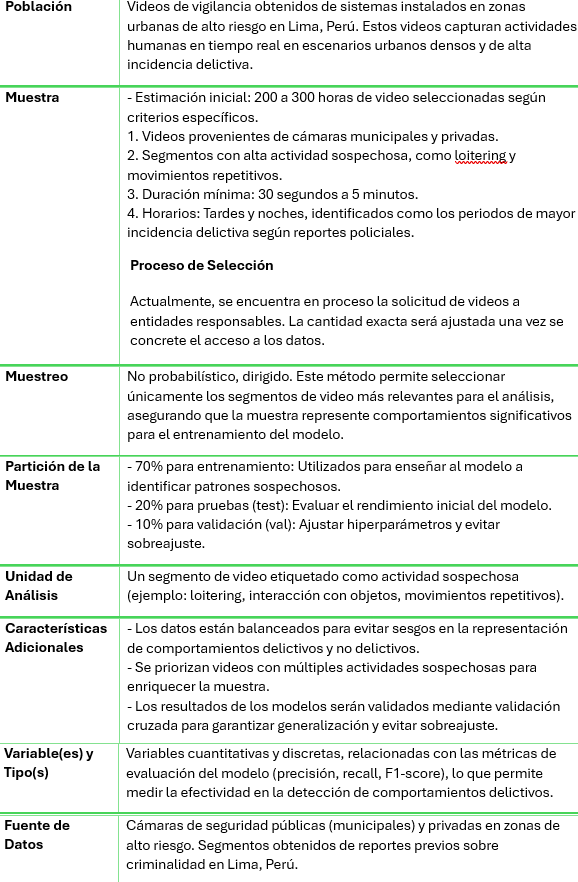
\includegraphics[width=0.7\textwidth]{TABLA MUESTRA.png} % Ruta y tamaño de la imagen
    \label{fig:ejemplo} % Etiqueta para referenciar la imagen
\end{figure}

\chapter{Operacionalización de variables}
Donde:
\begin{itemize}
    \item TP (True Positives): Casos correctamente clasificados como positivos.
    \item TN (True Negatives): Casos correctamente clasificados como negativos.
    \item FP (False Positives): Casos incorrectamente clasificados como positivos.
    \item FN (False Negatives): Casos incorrectamente clasificados como negativos.
\end{itemize}

\begin{figure}
    \centering
    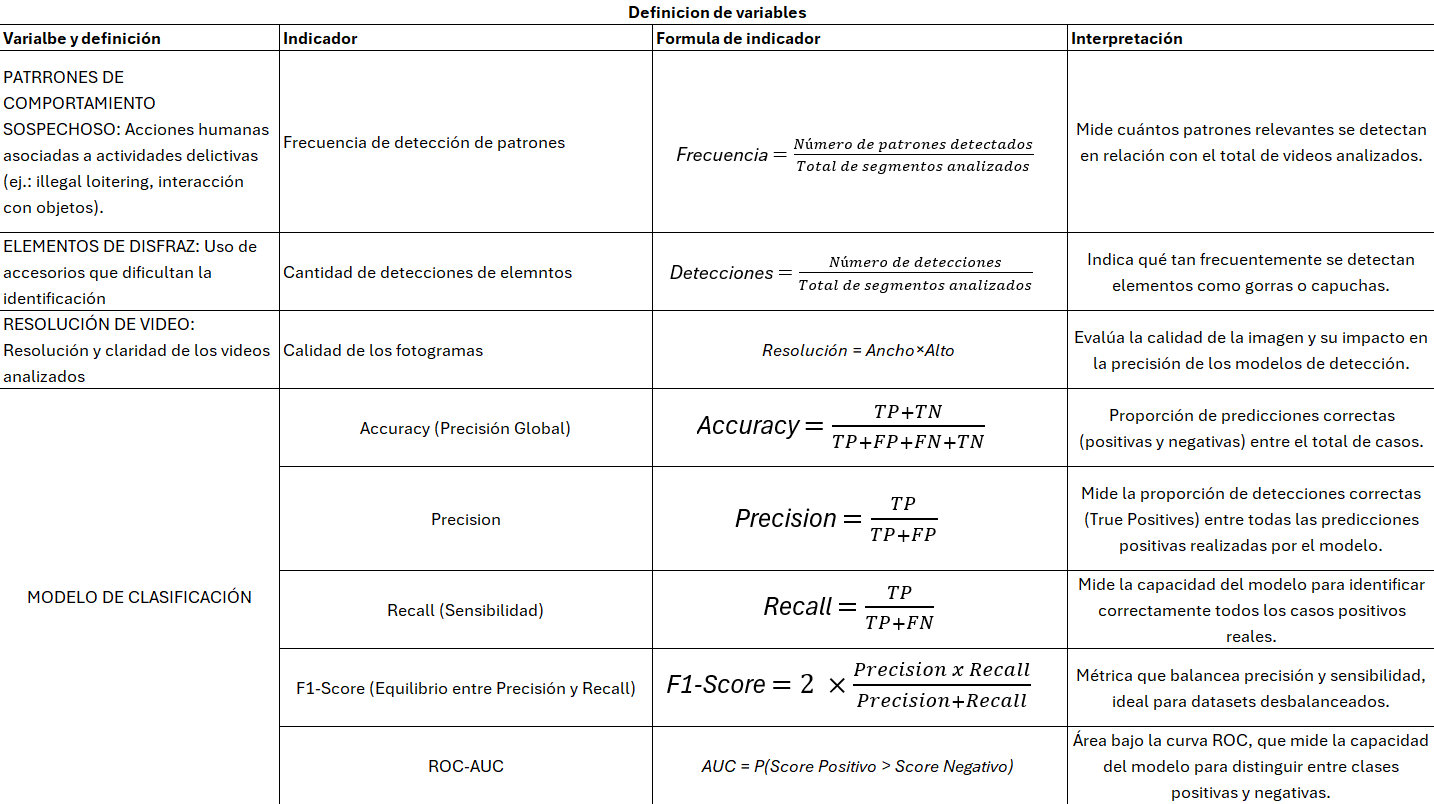
\includegraphics[width=1.1\linewidth]{tabla try.png}
\end{figure}

\chapter{Técnicas de Recolección de Datos}
La recolección de datos para esta investigación se basa en la obtención de videos de vigilancia provenientes de cámaras municipales en zonas urbanas de alto riesgo en Lima, Perú. Este proceso comienza con la identificación de áreas prioritarias, utilizando reportes estadísticos y policiales que reflejan las zonas con mayor incidencia delictiva. Una vez seleccionadas estas áreas, se identifican las cámaras municipales disponibles en dichas ubicaciones, evaluando su relevancia y calidad como fuente de datos.

Posteriormente, se elabora una solicitud formal dirigida a las municipalidades, explicando los objetivos de la investigación y detallando las especificaciones de los datos requeridos. Estas solicitudes garantizan el cumplimiento de normativas de privacidad y confidencialidad. Una vez enviadas, se realiza un seguimiento para negociar términos de acceso que permitan la utilización de los videos con fines investigativos.

Tras la recepción de los videos, estos son revisados para asegurar que cumplan con los estándares técnicos necesarios, como el formato (MP4 o AVI) y una resolución mínima de 720p. Este proceso asegura que los datos recolectados sean útiles y de calidad suficiente para entrenar los modelos de inteligencia artificial diseñados para detectar comportamientos sospechosos. Finalmente, los videos se preparan para el análisis, asegurando que estén listos para su preprocesamiento y segmentación en fragmentos relevantes.

\begin{figure}[h] % "h" indica que la imagen se coloque aproximadamente aquí
    \centering
    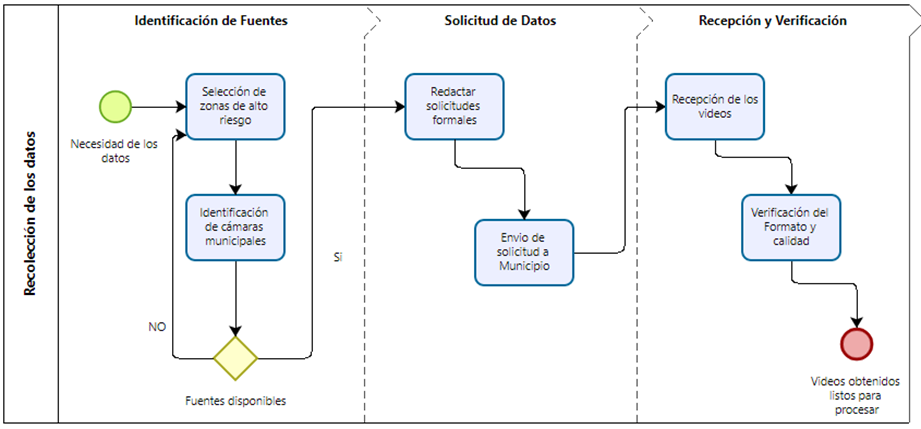
\includegraphics[width=1.0\textwidth]{proc.png} % Ruta y tamaño de la imagen
    \label{fig:ejemplo} % Etiqueta para referenciar la imagen
\end{figure}

\chapter{Técnicas para el Procesamiento y Análisis de la Información}
Para abordar el problema de la detección de comportamientos sospechosos en entornos urbanos, se seleccionó una metodología basada en los antecedentes más relevantes de la literatura científica. Los estudios de Sultani et al. (2018), Sun et al. (2021), y otros autores han demostrado la eficacia de enfoques híbridos que combinan aprendizaje profundo, extracción de características y segmentación en tiempo real para analizar datos visuales en entornos de vigilancia. Esta investigación adapta y expande estas metodologías para optimizar la precisión y robustez del sistema propuesto.


\begin{figure}[h] % "h" indica que la imagen se coloque aproximadamente aquí
    \centering
    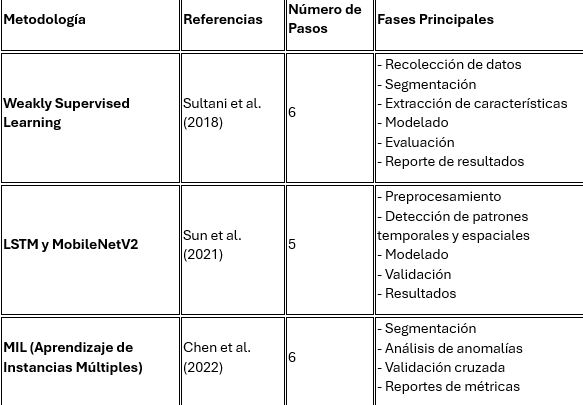
\includegraphics[width=1.0\textwidth]{proceso.png} % Ruta y tamaño de la imagen
    \label{fig:ejemplo} % Etiqueta para referenciar la imagen
\end{figure}

Se adaptó un enfoque híbrido basado en Weakly Supervised Learning y técnicas avanzadas de redes neuronales recurrentes para implementar la solución. La elección de esta metodología se fundamenta en su capacidad para manejar grandes volúmenes de datos visuales, adaptarse a escenarios urbanos complejos y proporcionar resultados en tiempo real, como se evidencia en los antecedentes citados.


\begin{figure}[h] % "h" indica que la imagen se coloque aproximadamente aquí
    \centering
    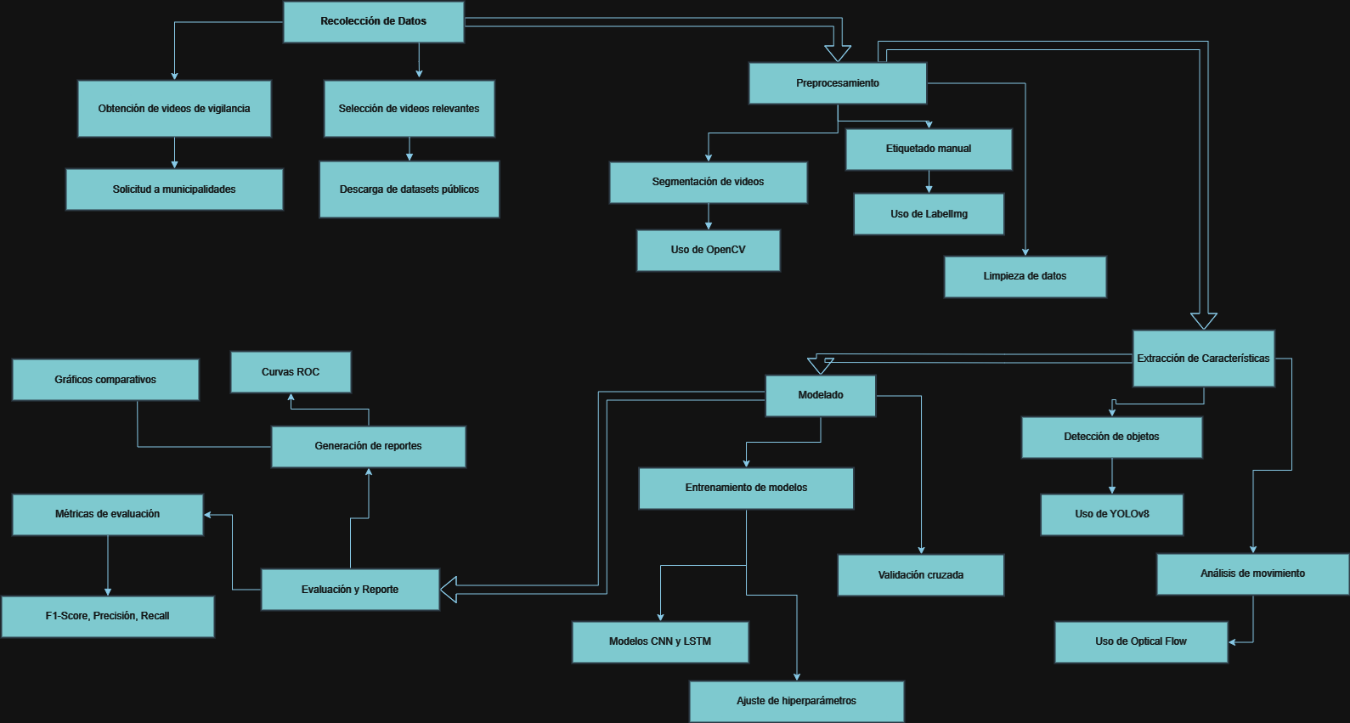
\includegraphics[width=0.8\textwidth]{propuesta.png} % Ruta y tamaño de la imagen
    \label{fig:ejemplo} % Etiqueta para referenciar la imagen
\end{figure}

\section{Recolección de Datos}
La primera etapa se enfoca en la obtención de videos relevantes para el análisis de comportamientos sospechosos en zonas urbanas de alto riesgo. Los datos se recopilarán de dos fuentes principales:
\begin{itemize}
    \item Cámaras municipales en zonas priorizadas mediante solicitudes formales a las municipalidades.
    \item Datasets públicos relevantes, como UCF-Crime, que contienen videos etiquetados de actividades anómalas.
\end{itemize}
Nuestro objetivo es asegurar una base de datos adecuada en términos de calidad, formato y cantidad, necesaria para el entrenamiento y validación de los modelos de inteligencia artificial.

\paragraph{\textit{Actividades}}

\subsubsection{Identificación de Fuentes}

\begin{itemize}
    \item Definir zonas urbanas de alto riesgo basadas en reportes policiales y estadísticas.
    \item Localizar cámaras municipales y privadas disponibles en esas zonas.
\end{itemize}

\subsubsection{Elaboración de Solicitudes}
\begin{itemize}
    \item Preparar solicitudes formales dirigidas a municipalidades y otras entidades responsables, explicando los objetivos de la investigación y el uso planificado de los videos.
\end{itemize}

\subsubsection{Revisión de Datasets Públicos}
\begin{itemize}
    \item Analizar datasets existentes como UCF-Crime y otros similares para complementar los datos municipales.
    \item Asegurar que los datos cumplan con los requisitos de calidad (formato MP4 o AVI, resolución mínima 720p).
\end{itemize}

\subsubsection{Recepción y Almacenamiento}
\begin{itemize}
    \item Centralizar los videos recolectados en un repositorio seguro.
    \item Organizar los datos por zonas, fechas y relevancia del contenido.
\end{itemize}


\paragraph{\textit{Herramientas Utilizadas}}

\subsubsection{Software}
\begin{itemize}
    \item Google Drive y herramientas similares para almacenamiento temporal.
    \item Excel/Google Sheets para la organización de los metadatos (ubicación, fecha, duración, calidad).
\end{itemize}

\subsubsection{Datasets Públicos}
\begin{itemize}
    \item UCF-Crime Dataset: Incluye videos etiquetados de actividades sospechosas.
\end{itemize}

\paragraph{\textit{Entregables}}

\subsubsection{Base de Datos Consolidada}
\begin{itemize}
    \item Videos organizados por zona y fecha.
    \item Identificación de videos relevantes para el análisis.
\end{itemize}

\subsubsection{Reporte de Calidad de los Datos}
\begin{itemize}
    \item Evaluación inicial de la calidad de los videos (formato, resolución, duración).
    \item Identificación de videos que requieren preprocesamiento adicional.
\end{itemize}



\section{Preprocesamiento}
En esta fase, los videos recolectados se preparan para el análisis. Este proceso incluye la limpieza de datos irrelevantes, la segmentación de los videos en fragmentos manejables y el etiquetado manual o semiautomático de eventos relevantes. El objetivo principal es garantizar que los datos estén listos para el entrenamiento de los modelos de inteligencia artificial.
Lo que se busca es optimizar la calidad de los datos y estructurarlos de manera que puedan ser utilizados eficazmente por los algoritmos de aprendizaje profundo.

\paragraph{\textit{Actividades}}

\subsubsection{Limpieza de Datos}

\begin{itemize}
    \item Verificar la resolución de los videos y descartar aquellos con calidad inferior a 720p.
    \item Eliminar segmentos de video que no contengan actividad humana relevante o que presenten problemas técnicos como ruido excesivo.
\end{itemize}


\subsubsection{Segmentación}
\begin{itemize}
    \item Dividir los videos en fragmentos más pequeños (30 segundos a 5 minutos) para facilitar el procesamiento y etiquetado.
    \item Utilizar herramientas como OpenCV para automatizar el proceso de segmentación.
\end{itemize}

\subsubsection{Etiquetado Manual}
Clasificar los fragmentos de video según categorías específicas como
\begin{itemize}
    \item Loitering: Comportamiento de permanencia prolongada.
    \item Interacción con objetos: Manipulación sospechosa de mochilas u otros elementos.
    \item Movimientos repetitivos: Indicativos de evasión o preparación para actividades delictivas.
\end{itemize}

\subsubsection{Normalización de Datos}
Asegurar que todos los videos segmentados tengan un formato estándar (e.g., MP4) y una resolución consistente para evitar problemas en el entrenamiento.


\paragraph{\textit{Herramientas Utilizadas}}

\subsubsection{Software}
\begin{itemize}
    \item OpenCV: Para la segmentación automática de videos.
    \item LabelImg: Para etiquetar manualmente los comportamientos sospechosos.
\end{itemize}

\subsubsection{Hardware}
\begin{itemize}
    \item Computadoras con capacidad para manejar procesamiento intensivo de video.
    \item Almacenamiento seguro para guardar los fragmentos procesados
\end{itemize}

\paragraph{\textit{Entregables}}

\subsubsection{Dataset Segmentado}
\begin{itemize}
    \item Fragmentos de video clasificados y organizados.
    \item Estructura clara para facilitar el acceso y uso en etapas posteriores.
\end{itemize}


\subsubsection{Reporte de Limpieza}
\begin{itemize}
    \item Detalle de los videos descartados y las razones (e.g., baja calidad, ausencia de actividad relevante).
\end{itemize}


\subsubsection{Anotaciones Etiquetadas}
\begin{itemize}
    \item Dataset enriquecido con etiquetas manuales, indicando eventos sospechosos.
\end{itemize}




\section{Extracción de Características}

En esta etapa, se identifican patrones visuales y temporales relevantes de los videos segmentados y etiquetados. Esto incluye analizar aspectos como la detección de objetos, trayectorias de movimiento y comportamientos anómalos. La extracción de características permite transformar los datos visuales en variables cuantificables que serán utilizadas en los modelos de aprendizaje.
El extraer información clave de los videos procesados es fundamental para optimizar el desempeño de los modelos de clasificación y predicción.


\paragraph{\textit{Actividades}}

\subsubsection{Análisis Visual}

\begin{itemize}
    \item Detectar objetos relevantes como gorras, capuchas o mochilas utilizando algoritmos avanzados como YOLOv8.
    \item Identificar posturas corporales sospechosas que puedan indicar comportamientos delictivos.
\end{itemize}


\subsubsection{Análisis Temporal}
\begin{itemize}
    \item Evaluar trayectorias de movimiento mediante Optical Flow para identificar patrones anómalos, como movimientos repetitivos o evasivos.
    \item Analizar la interacción entre individuos o con objetos en el espacio monitoreado.
\end{itemize}


\subsubsection{Conversión de Datos}
\begin{itemize}
    \item Transformar las características visuales y temporales extraídas en variables tabulares para su posterior uso en algoritmos de clasificación.
    \item Estandarizar los valores obtenidos para garantizar consistencia en el entrenamiento de los modelos.
\end{itemize}



\subsubsection{Validación de Características}
\begin{itemize}
    \item Realizar un análisis exploratorio de las características extraídas para verificar su relevancia y eliminar variables redundantes o no significativas.
\end{itemize}


\paragraph{\textit{Herramientas Utilizadas}}

\subsubsection{Software}
\begin{itemize}
    \item YOLOv8: Para la detección de objetos en tiempo real.
    \item Optical Flow: Para el análisis de movimientos en secuencias de video.
\end{itemize}

\subsubsection{Hardware}
\begin{itemize}
    \item GPU de alto rendimiento para acelerar los procesos de detección y análisis.
\end{itemize}

\paragraph{\textit{Entregables}}

\subsubsection{Dataset de Características}
\begin{itemize}
    \item Archivo tabular con las variables clave extraídas de los videos (e.g., número de objetos detectados, trayectorias de movimiento).
\end{itemize}

\subsubsection{Reporte de Análisis Exploratorio}
\begin{itemize}
    \item Resumen estadístico y visualización inicial de las características más relevantes.
\end{itemize}

\subsubsection{Variables Estandarizadas}
\begin{itemize}
    \item Conjunto de datos listo para el modelado, con valores normalizados y sin redundancias.
\end{itemize}


\section{Modelado}
Esta etapa se centra en la implementación de modelos de aprendizaje profundo y supervisado para la detección de comportamientos sospechosos. Utilizando características visuales y temporales extraídas en la fase previa, se entrenan y validan los modelos para garantizar que puedan identificar patrones sospechosos con alta precisión.
Lo que buscamos es diseñar y entrenar modelos robustos de aprendizaje que permitan analizar datos de vigilancia en tiempo real y emitir alertas precisas.


\paragraph{\textit{Actividades}}

\subsubsection{Selección de Modelos}

\begin{itemize}
    \item YOLOv8: Para la detección en tiempo real de objetos y posturas corporales.
    \item ConvLSTM: Para analizar secuencias temporales y detectar patrones anómalos.
    \item SVM (Support Vector Machines): Para clasificar eventos específicos con características predefinidas como gorras o movimientos repetitivos.
\end{itemize}


\subsubsection{Configuración del Entorno}
\begin{itemize}
    \item Frameworks como TensorFlow y PyTorch.
    \item Configuración de GPU para acelerar el entrenamiento.
\end{itemize}


\subsubsection{Entrenamiento de los Modelos}
Dividir el dataset en:
\begin{itemize}
    \item 70\% para entrenamiento.
    \item 20\% para pruebas.
    \item 10\% para validación.
\end{itemize}

Implementar optimizadores como Adam y SGD para ajustar los hiperparámetros de los modelos.

\subsubsection{Validación Cruzada}
\begin{itemize}
    \item Evaluar el desempeño de los modelos mediante validación cruzada para evitar el sobreajuste.
    \item Comparar el rendimiento de los modelos seleccionados utilizando el conjunto de validación.
\end{itemize}

\subsubsection{Ajuste de Hiperparámetros}
\begin{itemize}
    \item Ajustar parámetros como la tasa de aprendizaje, el número de capas y el tamaño del batch para maximizar la precisión del modelo.
\end{itemize}


\paragraph{\textit{Herramientas Utilizadas}}

\subsubsection{Software}
\begin{itemize}
    \item Frameworks: TensorFlow, PyTorch.
    \item Modelos: YOLOv8 para detección de objetos, ConvLSTM para secuencias temporales y SVM para clasificación específica.
\end{itemize}

\subsubsection{Hardware}
\begin{itemize}
    \item GPU de alto rendimiento para acelerar el entrenamiento.
\end{itemize}

\paragraph{\textit{Entregables}}

\subsubsection{Modelos Entrenados}
\begin{itemize}
    \item Algoritmos configurados y optimizados listos para pruebas en entornos simulados.
\end{itemize}


\subsubsection{Reporte de Desempeño}
\begin{itemize}
    \item Métricas de evaluación como precisión, recall, F1-Score, y curvas ROC
\end{itemize}


\subsubsection{Comparación de Modelos}
\begin{itemize}
    \item Gráficos comparativos que muestren el desempeño de cada modelo en el dataset.
\end{itemize}


\section{Evaluación y Reporte}
En esta etapa, se evalúan los modelos entrenados utilizando métricas estándar para medir su precisión y efectividad en la detección de comportamientos sospechosos. Además, se generan reportes detallados con gráficos y análisis comparativos que facilitan la interpretación de los resultados obtenidos.
Nuestro objetivo es validar el desempeño de los modelos entrenados y documentar los resultados de manera clara y comprensible para su análisis y futuras mejoras.



\paragraph{\textit{Actividades}}

\subsubsection{Evaluación del Modelo}

\begin{itemize}
    \item Precisión (Accuracy): Proporción de predicciones correctas.
    \item Recall: Capacidad del modelo para identificar correctamente eventos sospechosos.
    \item F1-Score: Balance entre precisión y recall.
    \item Curvas ROC y AUC: Medir el trade-off entre sensibilidad y especificidad.
\end{itemize}



\subsubsection{Análisis Comparativo}
\begin{itemize}
    \item Comparar el desempeño entre los diferentes modelos utilizados (e.g., YOLOv8, ConvLSTM, SVM).
    \item Identificar fortalezas y limitaciones de cada modelo en relación con los datos recolectados.
\end{itemize}



\subsubsection{Visualización de Resultados}
Dividir el dataset en:
\begin{itemize}
    \item Gráficos de barras: Comparación de precisión entre modelos.
    \item Curvas ROC: Evaluación de sensibilidad y especificidad.
    \item Mapas de calor: Identificación de áreas críticas en los videos.
\end{itemize}

\subsubsection{Documentación}
\begin{itemize}
    \item Métodos utilizados para la evaluación.
    \item Resultados obtenidos en cada métrica.
    \item Limitaciones identificadas y recomendaciones para mejoras futuras
\end{itemize}


\paragraph{\textit{Herramientas Utilizadas}}

\subsubsection{Software de visualización}
\begin{itemize}
    \item Matplotlib y Seaborn para gráficos comparativos.
    \item Scikit-learn para generación de curvas ROC y análisis de métricas.
\end{itemize}

\subsubsection{Frameworks de Evaluación}
\begin{itemize}
    \item TensorFlow y PyTorch para validación y generación de resultados.
\end{itemize}

\paragraph{\textit{Entregables}}

\subsubsection{Reporte de Métricas}
\begin{itemize}
    \item Tabla con resultados detallados para cada modelo (Precisión, Recall, F1-Score).
\end{itemize}


\subsubsection{Gráficos Comparativos}
\begin{itemize}
    \item Visualizaciones que muestren el desempeño relativo de los modelos.
\end{itemize}


\subsubsection{Informe Final}
\begin{itemize}
    \item Documento que resuma los métodos, resultados y conclusiones del proceso de evaluación.
\end{itemize}




\chapter{Análisis Comparativo de Estudios}
\begin{landscape}
\begin{longtable}{|p{5cm}|p{4cm}|p{3cm}|p{2cm}|p{3cm}|p{5cm}|}
    \hline
    \textbf{Estudio} & \textbf{Metodología} & \textbf{Base de Datos} & \textbf{Precisión} & \textbf{Comportamientos Detectados} & \textbf{Observaciones Clave} \\ \hline
    Proactive Headcount and Suspicious Activity Detection using YOLOv8 & YOLOv8 para detección en tiempo real & Videos públicos en lugares urbanos y eventos de multitudes & 88\% & Densidad de multitudes, identificación de armas y caídas & Enfocado en detección de comportamientos de riesgo en espacios concurridos. \\ \hline
    Suspicious Activity Detection using LSTM and MobileNetV2 & CNN (MobileNetV2) + LSTM para secuencias temporales & Vigilancia en áreas comerciales & 70-74\% & Merodeo, peleas, robos & Uso de secuencias para análisis temporal; ideal para vigilancia continua. \\ \hline
    Toward Trustworthy Human Suspicious Activity Detection & CNN + GRU + ConvLSTM & Dataset propio con actividades etiquetadas & CNN: 91.55\%, ConvLSTM: 88.73\% & Correr, pelear, disparar & Fusión de modelos para mejorar precisión en entornos dinámicos. \\ \hline
    Anomaly Detection Using Edge Computing in Video Surveillance & Computación en el borde + CNN & Datasets de tráfico y áreas concurridas & 85\% & Comportamientos anómalos en alta concurrencia & Optimizados para procesamiento en tiempo real con computación en el borde. \\ \hline
    Real-World Anomaly Detection in Surveillance Videos & MIL (aprendizaje de instancias múltiples) + CNN & 128 horas de videos de vigilancia con eventos anómalos & 86\% en promedio & Robo, pelea, movimientos sospechosos & Enfoque en anomalías en videos no recortados, útil en detección general. \\ \hline
    Deep Learning Based Real-time Pedestrian Recognition System & YOLO + Seguimiento de movimiento & Escenas urbanas en entornos con múltiples cámaras & No especificada; alta velocidad en seguimiento & Reconocimiento de peatones y seguimiento & Ideal para seguimiento continuo en vigilancia de seguridad. \\ \hline
    Suspicious Human Activity Recognition From Surveillance Videos Using Deep Learning & Time-Distributed CNN + Conv3D & Videos de vigilancia de situaciones comunes & CNN: 90.14\%, Conv3D: 88.23\% & Correr, golpear, disparar & Buena precisión en actividades de alta acción; útil en seguridad pública. \\ \hline
    An Integrated Framework for Detecting Suspicious Behaviors in Video Surveillance & Modelos de Markov para patrones de movimiento & Dataset propio y público para escenarios de vigilancia & No especificada; detección efectiva en loitering y objetos abandonados & Loitering, objetos abandonados & Adecuado para detección en entornos con alta interacción entre personas. \\ \hline
\end{longtable}
\end{landscape}



\section{Matriz de Consistencia}
\begin{landscape}
\begin{longtable}{| m{4cm} | m{7cm} | m{7cm} | m{7cm} |}
    \hline
    \multicolumn{4}{|c|}{\textbf{Título: Sistema predictivo de visión por computadora e IA para detección de comportamientos sospechosos y alertas tempranas en entornos urbanos}} \\ \hline
    \textbf{Aspecto} & \textbf{Problema} & \textbf{Objetivo} & \textbf{Variables} \\ \hline
    
    \textbf{Principal} & ¿Cómo puede un sistema de visión por computadora e inteligencia artificial prever y analizar comportamientos delictivos para emitir alertas tempranas y mejorar la seguridad en zonas urbanas de alto riesgo? & Desarrollar un sistema basado en IA y visión por computadora que permita detectar y predecir comportamientos delictivos en tiempo real, con el objetivo de emitir alertas tempranas para mejorar la seguridad en entornos urbanos. & \textbf{Dependiente}: Incidencia delictiva, percepción de seguridad. \newline \textbf{Independiente}: Implementación del sistema de visión por computadora e IA. \\ \hline
    
    \textbf{Específicos} & ¿Por qué no existen suficientes herramientas tecnológicas que permitan detectar comportamientos delictivos en tiempo real? & Diseñar algoritmos de visión por computadora para la identificación de posturas y elementos de disfraz como gorras o capuchas. & \textbf{Dependiente}: Eficacia en la identificación de comportamientos sospechosos. \newline \textbf{Independiente}: Uso de algoritmos de visión por computadora y detección de elementos de disfraz. \\ \hline
    
    & ¿Qué dificultades existen en el uso de simulaciones predictivas para predecir comportamientos delictivos? & Implementar un modelo predictivo que analice patrones de comportamiento sospechoso y determine la probabilidad de que ocurra un delito. & \textbf{Dependiente}: Precisión del modelo predictivo. \newline \textbf{Independiente}: Simulaciones predictivas y datos históricos de delitos. \\ \hline
    
    & ¿Cómo se pueden mejorar los sistemas de videovigilancia mediante algoritmos de IA? & Validar el sistema mediante pruebas en escenarios simulados y analizar su precisión en la emisión de alertas tempranas. & \textbf{Dependiente}: Capacidad de respuesta de las alertas. \newline \textbf{Independiente}: Algoritmos de IA y condiciones de prueba. \\ \hline
\end{longtable}
\end{landscape}

% Bibliografía
\section{Bibliografia}

\begin{itemize}
    \item Sun, T., Zhao, R., Tang, X., \& Xu, W. (2021). \textbf{\textit{Suspicious Human Activity Recognition From Surveillance Videos Using Deep Learning}}. \textit{Sensors and Actuators A: Physical}, \textbf{323}, 112633.

    \item Sultani, W., Chen, C., \& Shah, M. (2018). \textbf{\textit{Real-World Anomaly Detection in Surveillance Videos}}. In \textit{Proceedings of the IEEE Conference on Computer Vision and Pattern Recognition (CVPR)} (pp. 6479--6488).

    \item Zin, T., Win, Z., \& Myo, T. (2014). \textbf{\textit{An Integrated Framework for Detecting Suspicious Behaviors in Video Surveillance}}. \textit{International Journal of Advanced Computer Science and Applications}, \textbf{5}(2), 85--91.

    \item Redmon, J., Divvala, S., Girshick, R., \& Farhadi, A. (2016). \textbf{\textit{You Only Look Once: Unified, Real-Time Object Detection}}. In \textit{Proceedings of the IEEE Conference on Computer Vision and Pattern Recognition (CVPR)} (pp. 779--788).

    \item Chen, J., Wu, H., \& Yang, J. (2022). \textbf{\textit{Anomaly Detection Using Edge Computing in Video Surveillance}}. \textit{Journal of Visual Communication and Image Representation}, \textbf{87}, 103564.

    \item Hochreiter, S., \& Schmidhuber, J. (1997). \textbf{\textit{Long Short-Term Memory}}. \textit{Neural Computation}, \textbf{9}(8), 1735--1780.

    \item Gonzalez, R. C., \& Woods, R. E. (2018). \textbf{\textit{Digital Image Processing}} (4th ed.). Pearson Education.

    \item Krizhevsky, A., Sutskever, I., \& Hinton, G. E. (2012). \textbf{\textit{ImageNet Classification with Deep Convolutional Neural Networks}}. In \textit{Advances in Neural Information Processing Systems}, \textbf{25}, 1097--1105.

    \item Shi, W., Cao, J., Zhang, Q., Li, Y., \& Xu, L. (2016). \textbf{\textit{Edge Computing: Vision and Challenges}}. \textit{IEEE Internet of Things Journal}, \textbf{3}(5), 637--646.

    \item Dietterich, T. G., Lathrop, R. H., \& Lozano-Pérez, T. (1997). \textbf{\textit{Solving the Multiple Instance Problem with Axis-Parallel Rectangles}}. \textit{Artificial Intelligence}, \textbf{89}(1--2), 31--71.

    \item Cho, K., Merrienboer, B. V., Bahdanau, D., \& Bengio, Y. (2014). \textbf{\textit{On the Properties of Neural Machine Translation: Encoder-Decoder Approaches}}. \textit{arXiv Preprint}.

    \item Marras, C., Canning, C. G., \& Goldman, S. M. (2020). \textbf{\textit{Parkinson’s Disease Across Races and Ethnicities: A Global View}}. \textit{Movement Disorders}, \textbf{35}(10), 1747--1757.
\end{itemize}
    
\end{document}
